\textbf{4.1.1.} 一种康铜丝的横截面积为 $0.10\mathrm{mm}^2$ ，电阻率为 $4.9 \times 10^{-7}\Omega \cdot \mathrm{m}$ ，试问用它绕制一个 $6.0\Omega$ 的电阻，需要多长？

\vfill

\textbf{4.1.2.} 一条长为 $l$ 的导线, 它的横截面积 $A$ 和电导率 $\sigma$ 都是 $x$ 的函数, $x$ 是到一端 $a$ 的距离, 如图4.1.2所示. (1)试问这段导线的电阻 $R$ 如何表示? (2)若这导线是圆台形, $a$ 端的横截面是半径为 $a$ 的圆, $b$ 端的横截面是半径为 $b$ 的圆, 而 $\sigma$ 则是常数. 试求它的电阻.

图4.1.2
\begin{center}
    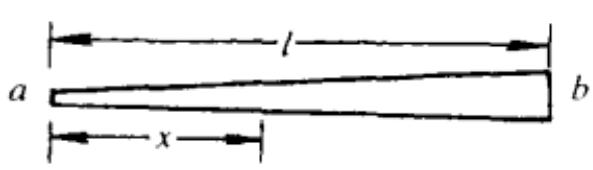
\includegraphics[width=0.5\linewidth]{figures/fig_4_1_2.jpg}
\end{center}

\vfill

\newpage

\textbf{4.1.3.} 一铜圆柱体长为 $l$ , 半径为 $a$ , 外面套有一个等长的共轴铜圆筒, 筒的内半径为 $b$ , 在柱与筒之间充满电导率为 $\sigma$ 的均匀物质, 如图 4.1.3 所示. 试求柱与筒之间的电阻.

\vfill

\textbf{4.1.4.} 一长为 $l = 10\mathrm{cm}$ 、内半径为 $r = 3.0\mathrm{cm}$ 的铜圆筒，竖立在玻璃片上，筒内盛满电阻率为 $\rho = 33\Omega \cdot \mathrm{cm}$ 的硫酸铜溶液；在溶液内轴线上，有一根直径为 $d = 1.0\mathrm{mm}$ 的导线，如图4.1.4所示。现在铜筒和导线间加上 $U = 2.0\mathrm{V}$ 的电压，试求电流 $I$ 。

\vfill

\newpage

\textbf{4.1.5.} 有两个电阻,并联时总电阻为 $2.4\Omega$ , 串联时总电阻是 $10\Omega$ . 试问这两个电阻各是多少?

\vfill

\textbf{4.1.6.} 试证明:一些电阻并联后的总电阻比它们中最小的电阻还要小.

\vfill

\newpage

\textbf{4.1.7.} 四个电阻 $R_{1}, R_{2}, R_{3}, R_{4}$ , 两种联法, 分别如图 4.1.7 所示. 设 $a, b$ 间的电阻为 $R_{ab}, c, d$ 之间的电阻为 $R_{cd}$ , (1) 试证明: $R_{cd} \leqslant R_{ab}$ ; (2) 在什么情况下, $R_{cd} = R_{ab}$ ?

图4.1.7
\begin{center}
    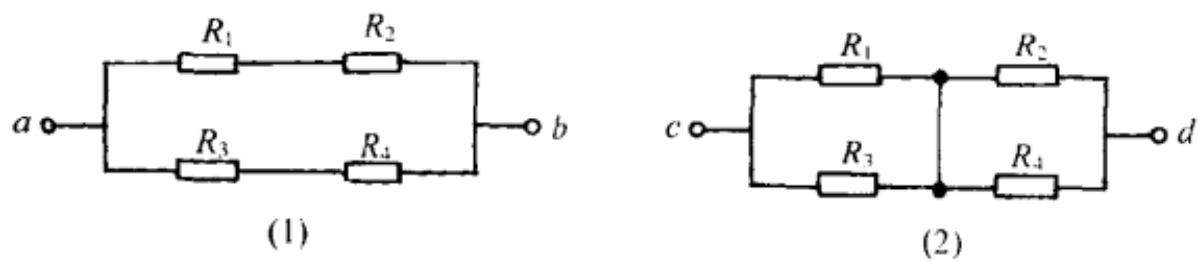
\includegraphics[width=0.5\linewidth]{figures/fig_4_1_7.jpg}
\end{center}

\vfill

\textbf{4.1.8.} 三个电阻 $r_1, r_2$ 和 $r_3$ 联接成三角形 $ABC$ , 另一电阻 $r_4$ , 一端接在三角形的顶点 $A$ , 另一端接在电阻 $r_1$ 上的 $D$ 点, $D$ 可以在 $r_1$ 上滑动, 如图4.1.8(1)

所示. 试证明: A、D 间电阻的最大值为 $(R_{AD})_{\max} = \frac{(r_{1} + r_{2} + r_{3})r_{4}}{r_{1} + r_{2} + r_{3} + 4r_{4}}$ .

图4.1.8(1)

图4.1.8(2)
\begin{center}
    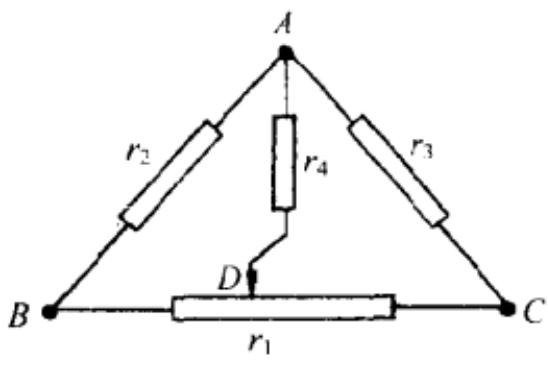
\includegraphics[width=0.5\linewidth]{figures/fig_4_1_8_1.jpg}
\end{center}
\begin{center}
    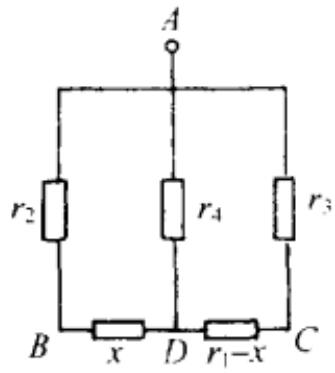
\includegraphics[width=0.5\linewidth]{figures/fig_4_1_8_2.jpg}
\end{center}

\vfill

\newpage

\textbf{4.1.9.} (1)两电阻 $R_{1}$ 和 $R_{2}$ 串联后加上电压 $U$ , 试分别求 $R_{1}$ 和 $R_{2}$ 上的电压 $U_{1}$ 和 $U_{2}$ ; (2)两电阻并联后通过的总电流为 $I$ , 试分别求通过 $R_{1}$ 和 $R_{2}$ 的电流 $I_{1}$ 和 $I_{2}$ .

\vfill

\textbf{4.1.10.} 一些电阻联接如图 4.1.10 (1) 所示, (1) 试求 a、b 间的电阻 $R_{ab}$ ; (2) 若 $4\Omega$ 电阻中的电流为 1A, 试求 a、b 间的电势差 $U_{ab}$ .
\begin{center}
    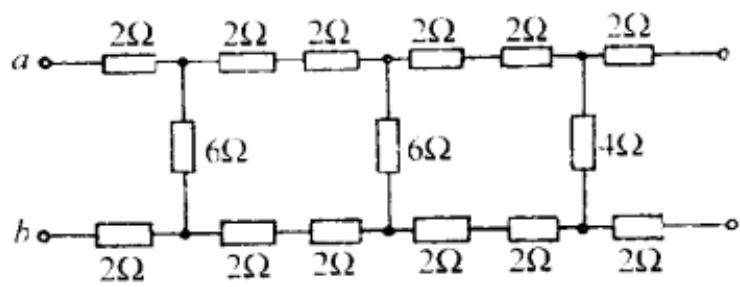
\includegraphics[width=0.5\linewidth]{figures/fig_4_1_10.jpg}
\end{center}

\vfill

\newpage

\textbf{4.1.11.} 三种已知电阻 $r_1, r_2$ 和 $r_3$ , 联接成一无穷长梯形电路, 如图 4.1.11 (1) 所示. 试求 $a, b$ 间的电阻 $R_{ab}$ .

图4.1.11(1)
\begin{center}
    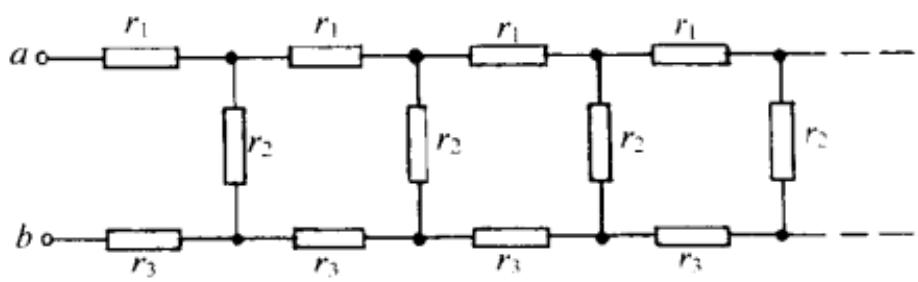
\includegraphics[width=0.5\linewidth]{figures/fig_4_1_11.jpg}
\end{center}

\vfill

\textbf{4.1.12.} 无轨电车速度的调节是依靠在直流电动机的回路中，串入不同数值的电阻，从而改变通过电动机的电流，使电动机的转速发生变化。例如，在回路中串接四个电阻 $R_{1}, R_{2}, R_{3}$ 和 $R_{4}$ ，再利用一些开关 $\mathrm{K}_{1}, \mathrm{K}_{2}, \mathrm{K}_{3}, \mathrm{K}_{4}$ 和 $\mathrm{K}_{5}$ ，使电阻分别串联或并联，以改变总电阻的数值，如图4.1.12所示。设 $R_{1} = R_{2} = R_{3} = R_{4} = 1.0\Omega$ ，试求下列三种情况下 $a, b$ 间的电阻 $R_{ab}$ ：(1) $\mathrm{K}_{1}, \mathrm{K}_{5}$ 接通， $\mathrm{K}_{2}, \mathrm{K}_{3}, \mathrm{K}_{4}$ 断开；(2) $\mathrm{K}_{2}, \mathrm{K}_{3}, \mathrm{K}_{5}$ 接通， $\mathrm{K}_{1}, \mathrm{K}_{4}$ 断开；(3) $\mathrm{K}_{1}, \mathrm{K}_{3}, \mathrm{K}_{4}$ 接通， $\mathrm{K}_{2}, \mathrm{K}_{5}$ 断开。




图4.1.12
\begin{center}
    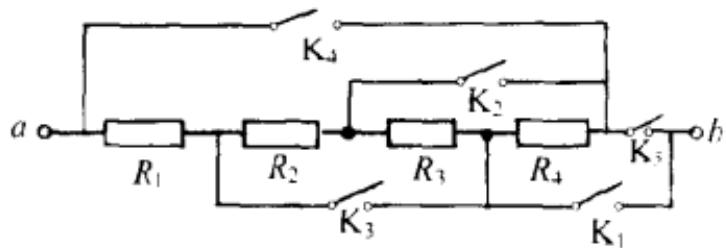
\includegraphics[width=0.5\linewidth]{figures/fig_4_1_12_1.jpg}
\end{center}
\begin{center}
    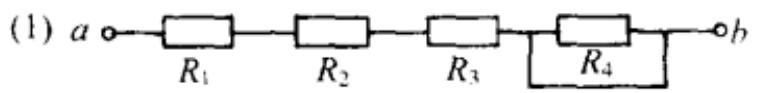
\includegraphics[width=0.5\linewidth]{figures/fig_4_1_12_2.jpg}
\end{center}
\begin{center}
    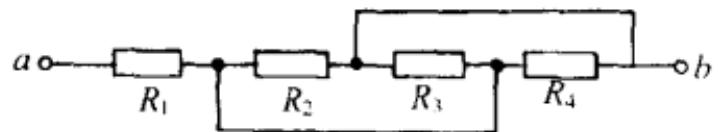
\includegraphics[width=0.5\linewidth]{figures/fig_4_1_12_3.jpg}
\end{center}
\begin{center}
    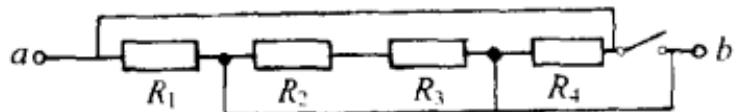
\includegraphics[width=0.5\linewidth]{figures/fig_4_1_12_4.jpg}
\end{center}

\vfill

\newpage

\textbf{4.1.13.} 图 4.1.13 是电学实验或仪器中调节电阻(从而可以用来调节电压或电流)的装置, 其中 R 是一个较大的电阻, r 是一个较小的电阻, R 和 r 都可以改变. 试证明: 当 $R \gg r$ 时, r 是粗调, R 是细调(即 r 改变某一数值时, a、b 间的电阻 $R_{ab}$ 改变较大; 而 R 改变同一数值时, $R_{ab}$ 则改变较小).

图4.1.13
\begin{center}
    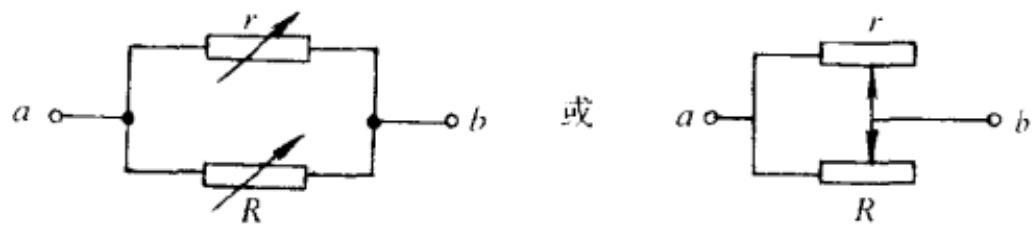
\includegraphics[width=0.5\linewidth]{figures/fig_4_1_13.jpg}
\end{center}

\vfill

\textbf{4.1.14.} 四个电阻联接如图 4.1.14(1)，已知 $R_{1}=R_{2}=8\Omega, R_{3}=4\Omega, R_{4}=2\Omega$ ，试求 a、b 间的电阻 $R_{ab}$ .

图 4.1.14(1)

图4.1.14(2)
\begin{center}
    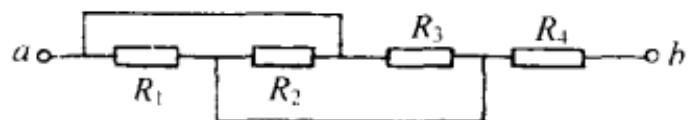
\includegraphics[width=0.5\linewidth]{figures/fig_4_1_14_1.jpg}
\end{center}
\begin{center}
    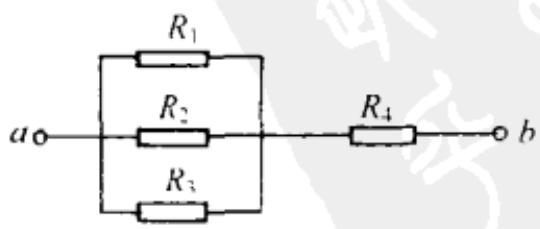
\includegraphics[width=0.5\linewidth]{figures/fig_4_1_14_2.jpg}
\end{center}

\vfill

\newpage

\textbf{4.1.15.} 五个已知电阻 $R_{1}, R_{2}, R_{3}, R_{4}$ 和 $R_{5}$ 联接如图4.1.15(1). 试求 $a, b$ 间的电阻 $R_{ab}$ .

图4.1.15(1)

图4.1.15(2)
\begin{center}
    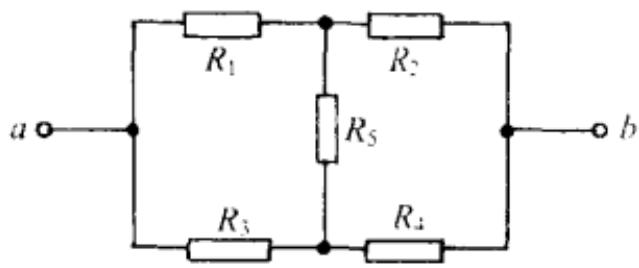
\includegraphics[width=0.5\linewidth]{figures/fig_4_1_15_1.jpg}
\end{center}
\begin{center}
    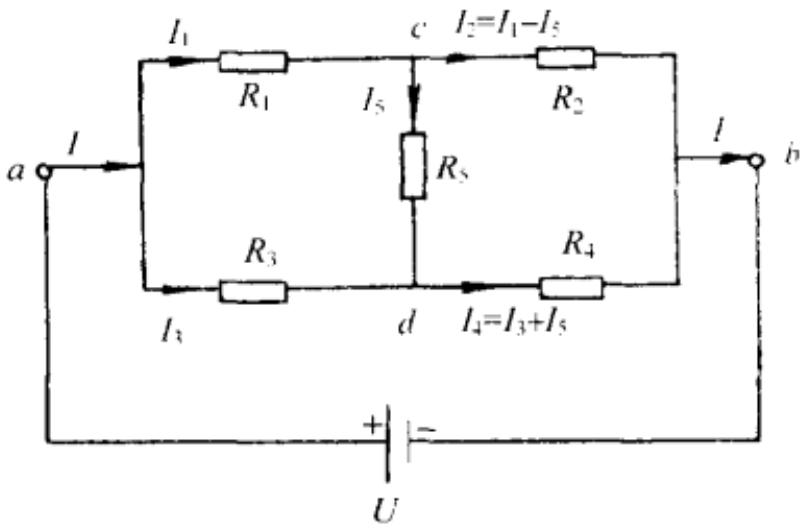
\includegraphics[width=0.5\linewidth]{figures/fig_4_1_15_2.jpg}
\end{center}

\vfill

\textbf{4.1.16.} 一些相同的电阻 r，分别联成如图 4.1.16 中所示的三种电路(1)、(2)和(3).试求每种电路 a、b 间的电阻 $R_{ab}$ .

(1)


(2)
图4.1.16
\begin{center}
    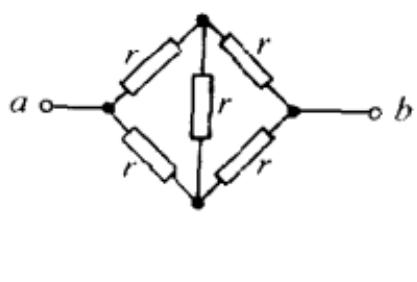
\includegraphics[width=0.5\linewidth]{figures/fig_4_1_16_1.jpg}
\end{center}
\begin{center}
    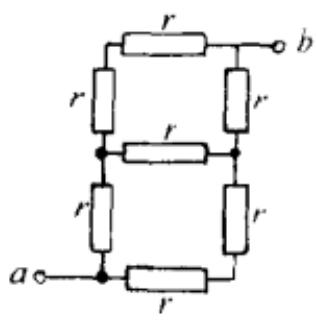
\includegraphics[width=0.5\linewidth]{figures/fig_4_1_16_2.jpg}
\end{center}
\begin{center}
    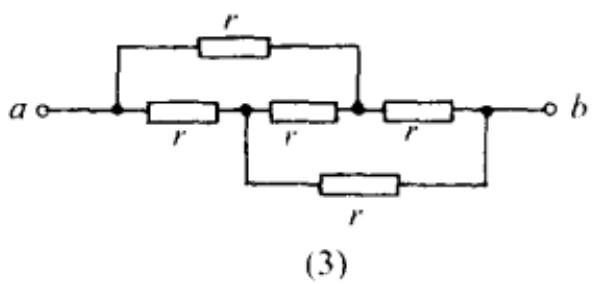
\includegraphics[width=0.5\linewidth]{figures/fig_4_1_16_3.jpg}
\end{center}

\vfill

\newpage

\textbf{4.1.17.} 试证明: 在 $R_{1}/R_{2}=R_{3}/R_{4}$ 的条件下, 图 4.1.17 中三个电路的 a、b 间的电阻 $R_{ab}$ 都相等.


(1)

(3)
图4.1.17
\begin{center}
    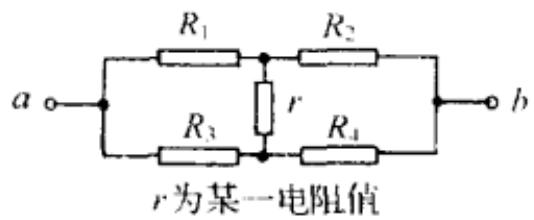
\includegraphics[width=0.5\linewidth]{figures/fig_4_1_17_1.jpg}
\end{center}
\begin{center}
    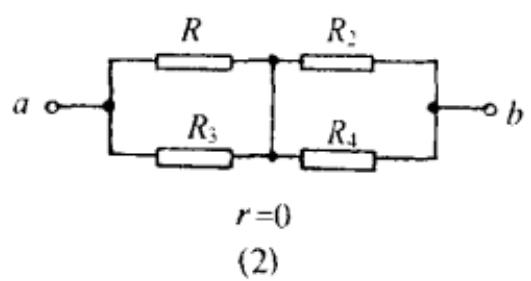
\includegraphics[width=0.5\linewidth]{figures/fig_4_1_17_2.jpg}
\end{center}
\begin{center}
    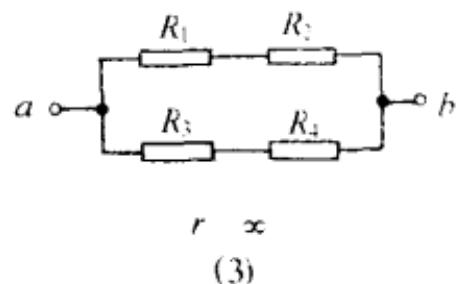
\includegraphics[width=0.5\linewidth]{figures/fig_4_1_17_3.jpg}
\end{center}

\vfill

\textbf{4.1.18.} 五个电阻联接如图 4.1.18, 其中电阻都已知. (1) 试求 a、b 间的电阻 $R_{ab}$ ; (2) 当 $R_{1}=4\Omega, R_{2}=2\Omega, R=1\Omega$ 时, $R_{ab}=?$ (3) 若拆去 R, 则 $R_{ab}=?$
\begin{center}
    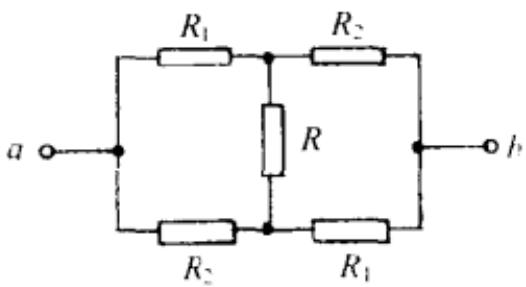
\includegraphics[width=0.5\linewidth]{figures/fig_4_1_18.jpg}
\end{center}

\vfill

\newpage

\textbf{4.1.19.} 六个相同的电阻 r 联接成如图 4.1.19 的电路, 试求 a、b 间的电阻 $R_{ab}$ 以及 a、c 间的电阻 $R_{ac}$ .
\begin{center}
    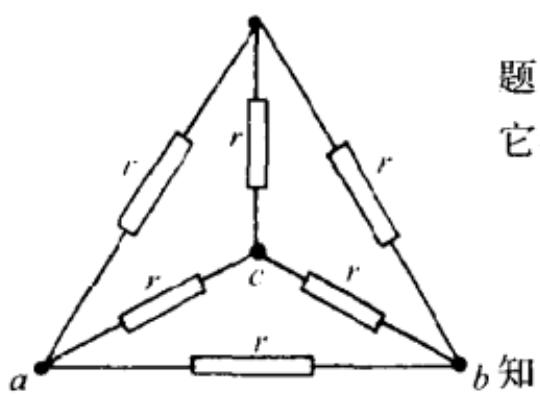
\includegraphics[width=0.5\linewidth]{figures/fig_4_1_19.jpg}
\end{center}

\vfill

\textbf{4.1.20.} 八个相同的电阻 r 联接成如图 4.1.20(1) 的电路, 试求: (1)a、b 间的电阻 $R_{ab}$ ; (2)a、c 间的电阻 $R_{ac}$ ; (3)a、d 间的电阻 $R_{ad}$ .

图4.1.20(1)

图4.1.20(2)
\begin{center}
    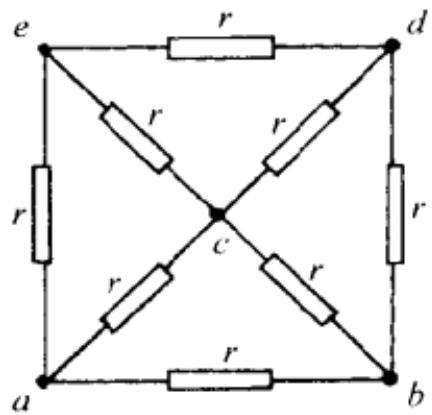
\includegraphics[width=0.5\linewidth]{figures/fig_4_1_20_1.jpg}
\end{center}
\begin{center}
    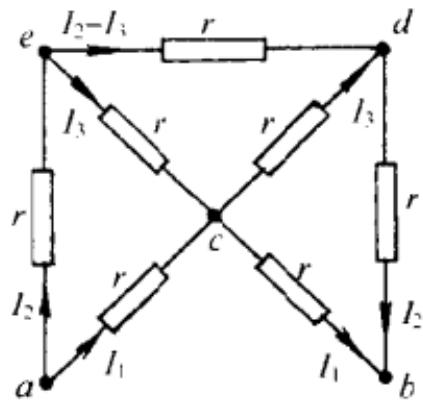
\includegraphics[width=0.5\linewidth]{figures/fig_4_1_20_2.jpg}
\end{center}

\vfill

\newpage

\textbf{4.1.21.} 十二个相同的电阻 r 联接成如图 4.1.21 (1) 的电路, 试求: (1) a、b 间的电阻 $R_{ab}$ ; (2) a、c 间的电阻 $R_{ac}$ ; (3) a、d 间的电阻 $R_{ad}$ ; (4) a、e 间的电阻 $R_{ae}$ .

\vfill

\textbf{4.1.22.} 图4.1.22(1)中的 X 和 Y 都是由电阻联接而成的电路. 试论证: 当 a、b 两端加上电压时, 如果 c、d 两点的电势相等(即电阻 r 中的电流为零), 则 a、b 两点间的电阻便与 r 无关.


图4.1.22(1)
图4.1.22(2)

【论证】图4.1.22(1)中的 $X$ 和 $Y$ 经过简化后， $a, b$ 间的电路最终可以化成图4.1.22(2)所示的电路，这是一个电桥电路。在 $a, b$ 间加上电压时， $c, d$ 间电势差为零，即 $r$ 中的电流为零，这时的电桥便是平衡电桥。根据前面4.1.15题后的讨论二，这时 $a, b$ 间的电阻为

$$
R _ {a b} = \frac {(R _ {1} + R _ {2}) R _ {3}}{R _ {1} + R _ {3}}
$$

它与电阻 r 无关.
\begin{center}
    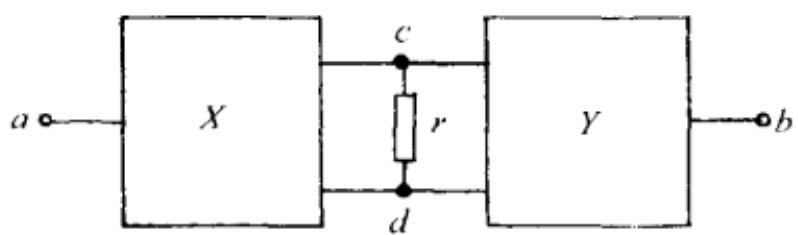
\includegraphics[width=0.5\linewidth]{figures/fig_4_1_22_1.jpg}
\end{center}
\begin{center}
    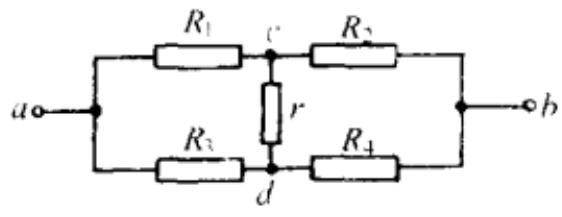
\includegraphics[width=0.5\linewidth]{figures/fig_4_1_22_2.jpg}
\end{center}

\vfill

\newpage

\textbf{4.1.23.} 试用前面 4.1.22 题的讨论中所讲的对称性原则解 4.1.19 题(即求

图 4.1.19 中 a、b 间的电阻 $R_{ab}$ 以及 a、c 间的电阻 $R_{ac}$ .

图4.1.19

图4.1.23
\begin{center}
    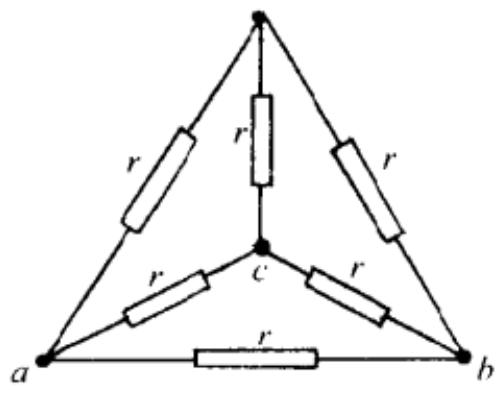
\includegraphics[width=0.5\linewidth]{figures/fig_4_1_23_1.jpg}
\end{center}
\begin{center}
    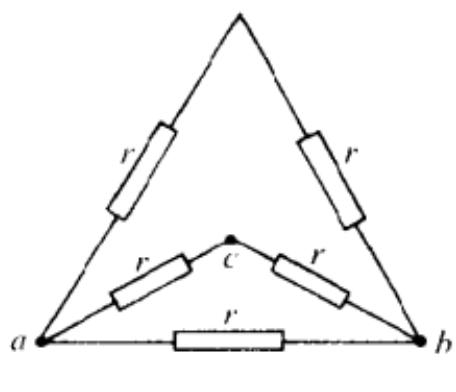
\includegraphics[width=0.5\linewidth]{figures/fig_4_1_23_2.jpg}
\end{center}

\vfill

\textbf{4.1.24.} 试用前面 4.1.22 题的讨论中所讲的对称性原则解 4.1.20 题, 即求图 4.1.20 中 (1) a、b 间的电阻 $R_{ab}$ ; (2) a、c 间的电阻 $R_{ac}$ ; (3) a、d 间的电阻 $R_{ad}$ .

图4.1.20

图4.1.24(1)
\begin{center}
    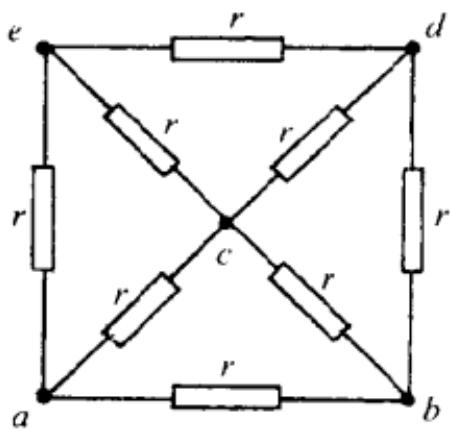
\includegraphics[width=0.5\linewidth]{figures/fig_4_1_24_1.jpg}
\end{center}
\begin{center}
    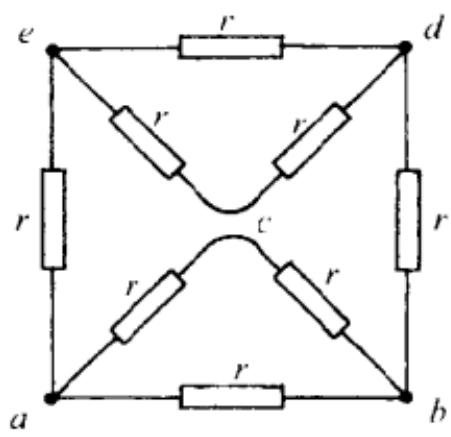
\includegraphics[width=0.5\linewidth]{figures/fig_4_1_24_2.jpg}
\end{center}

\vfill

\newpage

\textbf{4.1.25.} 试用前面 4.1.22 题的讨论中所讲的对称性原则解 4.1.21 题, 即求图 4.1.21 中 (1) $a$ 、 $b$ 间的电阻 $R_{ab}$ ; (2) $a$ 、 $c$ 间的电阻 $R_{ac}$ ; (3) $a$ 、 $d$ 间的电阻 $R_{ad}$ ; (4) $a$ 、 $e$ 间的电阻 $R_{ae}$ .

\vfill

\textbf{4.1.26.} 12个相同的电阻 $r$ 联接成每边为两个 $r$ 的正方格子，如图4.1.26所示.试求两对角 $a, b$ 间的电阻 $R_{ab}$ .

\vfill

\newpage

\textbf{4.1.27.} 12个相同的电阻 $r$ 联接成一个立方框架，如图4.1.27(1)所示.试求两对角 $a, d$ 之间的电阻 $R_{ad}$ .

图4.1.27(1)

图4.1.27(2)
\begin{center}
    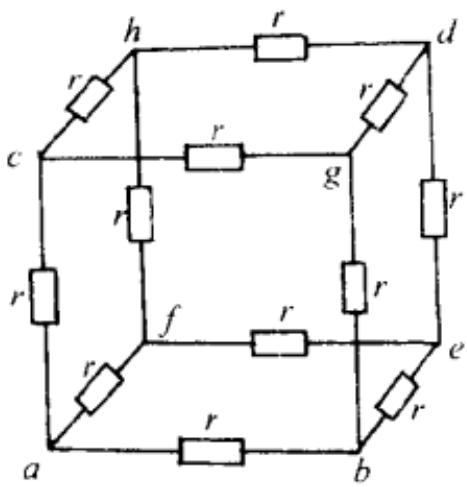
\includegraphics[width=0.5\linewidth]{figures/fig_4_1_27_1.jpg}
\end{center}
\begin{center}
    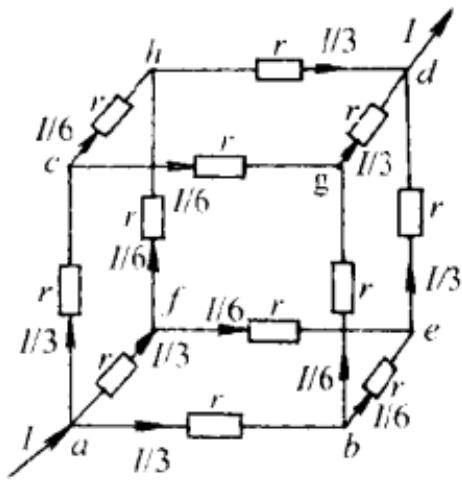
\includegraphics[width=0.5\linewidth]{figures/fig_4_1_27_2.jpg}
\end{center}

\vfill

\textbf{4.1.28.} 6个相同的电阻 r 联接成正六边形, 另外 6 个相同的电阻 $\frac{r}{n}$ 分别联接每个顶角和中心, 如图 4.1.28(1) 所示. 试求对角 a、b 间的电阻 $R_{ab}$ .

图4.1.28(1)

图 4.1.28(2)
\begin{center}
    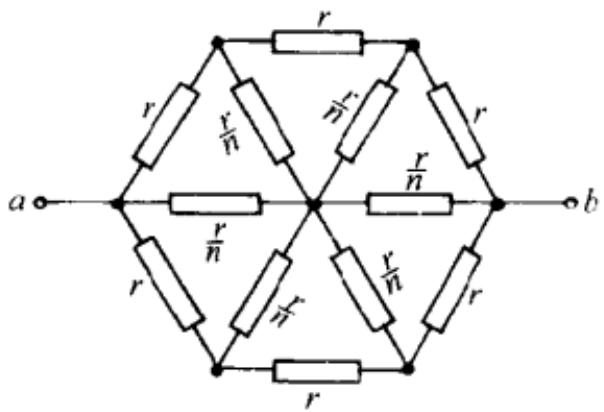
\includegraphics[width=0.5\linewidth]{figures/fig_4_1_28_1.jpg}
\end{center}
\begin{center}
    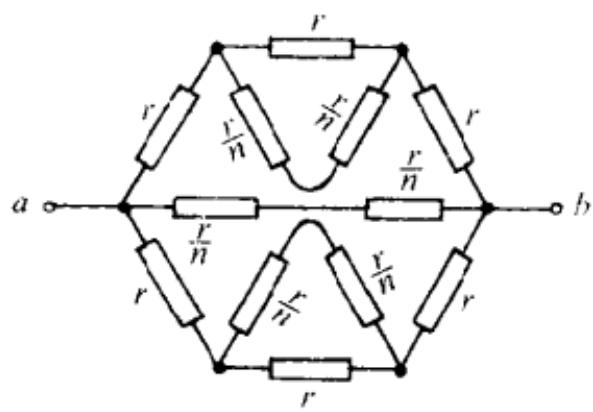
\includegraphics[width=0.5\linewidth]{figures/fig_4_1_28_2.jpg}
\end{center}

\vfill

\newpage

\textbf{4.1.29.} 24个相同的电阻 $r$ ，联接成每边三个电阻的正方格子，如图4.1.29(1)所示.试求对角 $a, b$ 间的电阻 $R_{ab}$ .

图4.1.29(1)

图4.1.29(2)
\begin{center}
    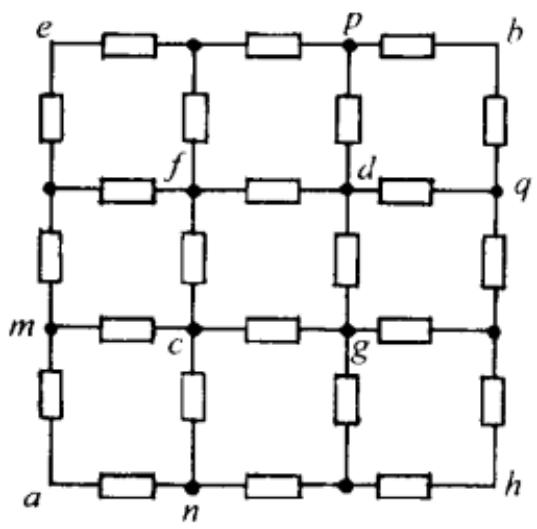
\includegraphics[width=0.5\linewidth]{figures/fig_4_1_29_1.jpg}
\end{center}
\begin{center}
    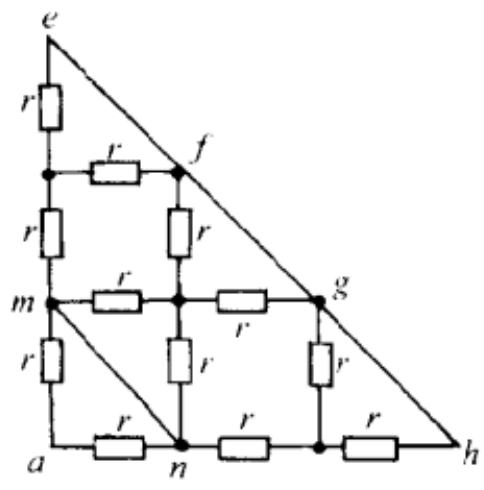
\includegraphics[width=0.5\linewidth]{figures/fig_4_1_29_2.jpg}
\end{center}

\vfill

\textbf{4.1.30.} 无穷多个相同的电阻, 每个都是 r, 联接成一个无穷大的平面正方格子, 如图 4.1.30 所示. 试论证: 相邻的两个节点 (如图 4.1.30 中的 a 和 b) 之间的电阻为 $\frac{r}{2}$ .

图4.1.30

【论证】设在 $a$ 点有电流 $I$ 流入这格子，则根据对称性，与 $a$ 相联的四个电阻中的电流便都是 $\frac{I}{4}$ ；同样，如果在 $b$ 点有电流 $I$ 流出这格子，则与 $b$ 相联的四个电阻中的电流便都是 $\frac{I}{4}$ 。若从 $a$ 流入 $I$ ，同时从 $b$ 流出 $I$ ，则根据叠加原理①， $a, b$ 间的那个电阻 $r$ 中的电流便为 $\frac{I}{4} + \frac{I}{4} = \frac{I}{2}$ 。因此，若在 $a, b$ 间加上电压 $U$ ，使电流 $I$ 从 $a$ 流入，从 $b$ 流出，便有

$$
U = \frac {I}{2} r = I R _ {a b}
$$

式中 $R_{ab}$ 为图4.1.30中 $a, b$ 间的电阻，由上式得

$$
R _ {a b} = \frac {r}{2}.
$$
\begin{center}
    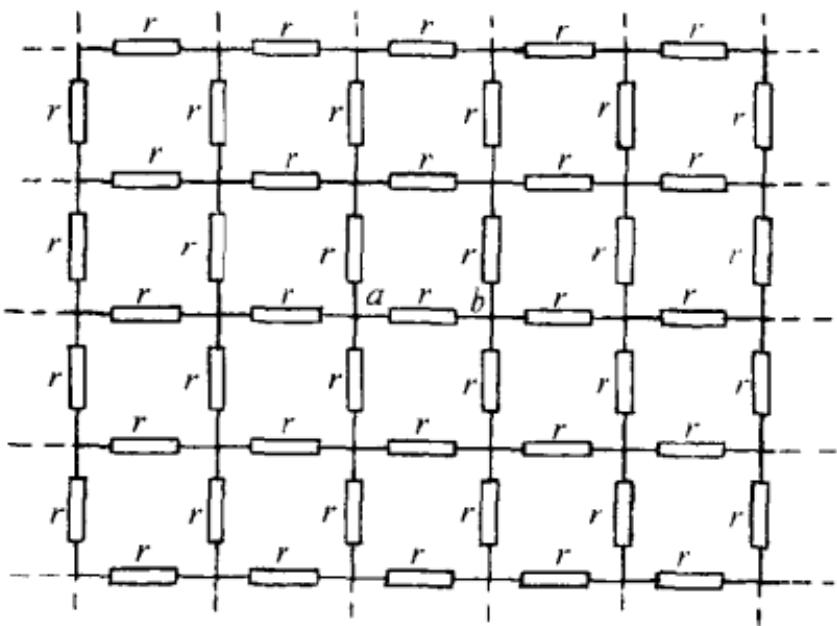
\includegraphics[width=0.5\linewidth]{figures/fig_4_1_30.jpg}
\end{center}

\vfill

\newpage

\textbf{4.1.31.} 三根等长的均匀电阻丝,电阻均为 r,联接成球形网架,如图 4.1.31 所示.试分别求 a、b 之间的电阻 $R_{ab}$ 和 a、c 之间的电阻 $R_{ac}$ .

\vfill

\textbf{4.1.32.} 三个电阻 $R_{1}, R_{2}, R_{3}$ 联接成三角形, 如图 4.1.32 的 (1) 所示; 另有三个电阻 $r_{1}, r_{2}, r_{3}$ 联接成星形, 如图 4.1.32 的 (2) 所示. 如果这两种联法的 1 与 2 之间, 2 与 3 之间, 3 与 1 之间的电阻都分别相等, 则 (1) 和 (2) 便互为等效电路. 在解决复杂电路问题时, 一个三角形电路 (1) 可以用它的星形等效电路 (2) 代替; 反之, 一个星形电路 (2) 也可以用它的三角形等效电路 (1) 代替. (1) 设三角形电路的电阻 $R_{1}, R_{2}$ 和 $R_{3}$ 均已知, 试求它的星形等效电路的电阻 $r_{1}, r_{2}$ 和 $r_{3}$ ; (2) 设星形电路的电阻 $r_{1}, r_{2}$ 和 $r_{3}$ 均已知, 试求它的三角形等效电路的电阻 $R_{1}, R_{2}$ 和 $R_{3}$ .


图4.1.32
\begin{center}
    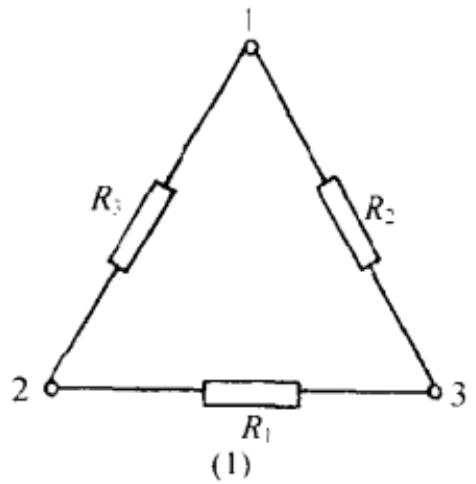
\includegraphics[width=0.5\linewidth]{figures/fig_4_1_32_1.jpg}
\end{center}
\begin{center}
    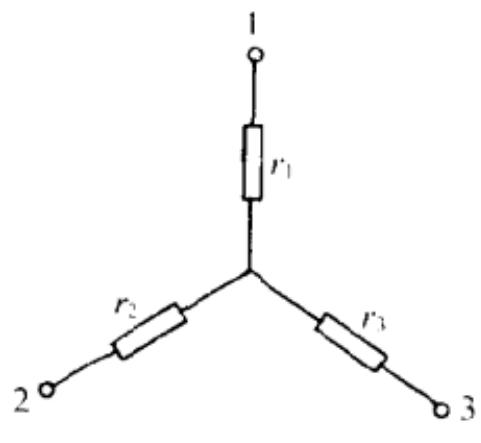
\includegraphics[width=0.5\linewidth]{figures/fig_4_1_32_2.jpg}
\end{center}

\vfill

\newpage

\textbf{4.1.33.} 试用前面 4.1.32 题的星形与三角形等效电路(也叫做 Y- $\Delta$ 变换)的方法求解前面的 4.1.15 题[即求图 4.1.15(1) 中 a、b 间的电阻 $R_{ab}$ ].

图4.1.15(1)

图4.1.33
\begin{center}
    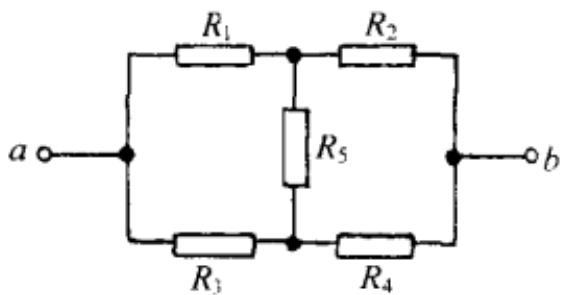
\includegraphics[width=0.5\linewidth]{figures/fig_4_1_33_1.jpg}
\end{center}
\begin{center}
    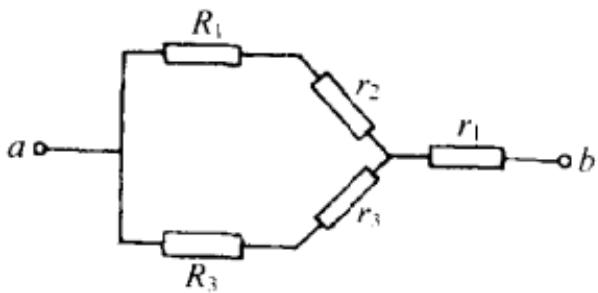
\includegraphics[width=0.5\linewidth]{figures/fig_4_1_33_2.jpg}
\end{center}

\vfill

\textbf{4.1.34.} 六根电阻丝, 长度和外形都相同, 联接成如图 4.1.34 所示的正四面体形的框架. 已知这六根电阻丝中有五根的电阻相同, 都是 $2\Omega$ , 另一根的电阻则比 $2\Omega$ 差很多. 试用测量电阻的欧姆表对这框架最多作三次测量, 以找出这根电阻不同的电阻丝.

\vfill

\newpage

\textbf{4.1.35.} 一个暗盒有四条导线接到外面, 如图 4.1.35(1) 所示. 已知盒内有四个相同的电阻, 每个电阻都是 $r$ . 现在测得每两个接头之间的电阻分别为 $R_{12} = R_{23} = R_{34} = R_{41} = \frac{r}{2}, R_{13} = r, R_{24} = 0$ . 试根据这些数据画出盒内四个电阻与四条导线的联接图.

图4.1.35(1)

图4.1.35(2)
\begin{center}
    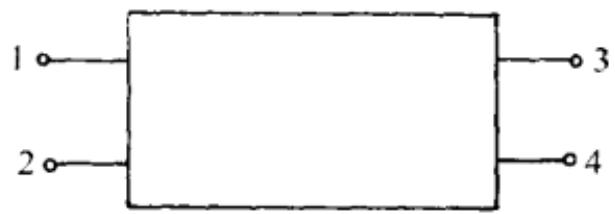
\includegraphics[width=0.5\linewidth]{figures/fig_4_1_35_1.jpg}
\end{center}
\begin{center}
    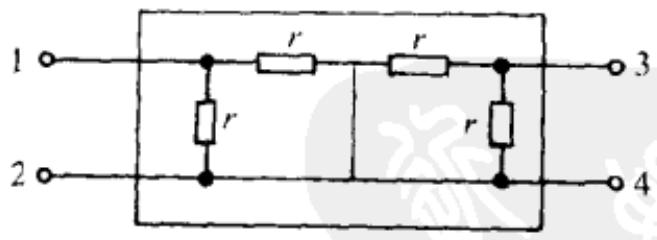
\includegraphics[width=0.5\linewidth]{figures/fig_4_1_35_2.jpg}
\end{center}

\vfill

\textbf{4.1.36.} 一电动机的磁绕组在温度为 $20^{\circ}\mathrm{C}$ 时的电阻为 $54\Omega$ ，它运行一段时间后，磁绕组的电阻变为 $60\Omega$ .已知磁绕组是由电阻温度系数为 $3.93\times 10^{-3}\mathrm{C}^{-1}$ 的铜丝绕成的，试求这时磁绕组的温度.

\vfill

\newpage

\textbf{4.2.1.} 在两层楼道之间安装一盏电灯，试设计一个线路，使得在楼上和楼下都能开关这电灯.
\begin{center}
    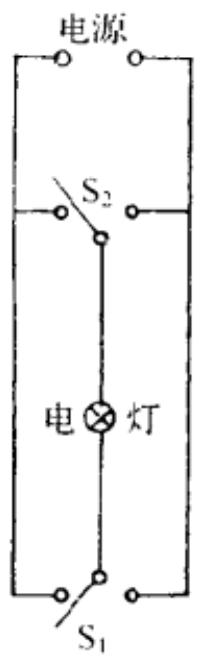
\includegraphics[width=0.5\linewidth]{figures/fig_4_2_1.jpg}
\end{center}

\vfill

\textbf{4.2.2.} 一分压器电路如图 4.2.2 所示, 已知 $R_{1}=4.3k\Omega$ , U=12V, 现在要使 c、d 间的电压为 2.0V, 试求 $R_{2}$ .

\vfill

\newpage

\textbf{4.2.3.} 变阻器可用做分压器，用法如图 4.2.3 所示， $\varepsilon$ 是电源的电动势，R 是

变阻器的电阻， $r$ 是负载电阻， $c$ 是 $R$ 上的滑动接头. 只要滑动 $c$ ，就可以得到从零到 $\varepsilon$ 之间的任何电压（电源的内阻很小，可略去不计). 设 $R$ 的长度为 $ab = l, R$ 上各处单位长度的电阻都相同， $a, c$ 之间的长度为 $ac = x$ ，试求加到 $r$ 上的电压 $U$ 与 $x$ 的关系.

\vfill

\textbf{4.2.4.} 一电路如图 4.2.4 所示,电阻 $R_{1}$ 、 $R_{2}$ 和 $R_{3}$ 以及电源的电动势 $\varepsilon$ 都已知,电源的内阻可略去不计.(1)试求通过安培计 A 的电流 $I_{A}$ ;(2)试证明:当电源和安培计互换位置后,安培计的读数不变.

\vfill

\newpage

\textbf{4.2.5.} 一安培计的电阻为 $R_A$ ，一伏特计的电阻为 $R_V$ ，用它们来测量电阻 $R$ ，有两种接法，分别如图4.2.5的(1)和(2)所示。这两种接法都用 $\frac{U}{I}$ 计算电阻，这里 $U$ 是伏特计测得的电压， $I$ 是安培计测得的电流。试求每种接法的误差（即 $\frac{U}{I}$ 与 $R$ 的百分误差）。如不需精确测定 $R$ ，且 $R$ 的范围大致知道，试问哪种接法较好？

$$
U = U _ {R}
$$

\vfill

\textbf{4.2.6.} 量程为 150V 的伏特计,电阻为 $20k\Omega$ , 当它与一个高电阻串联后接到 110V 电压上, 它的读数为 5.0V. 试求 R 的值.

\vfill

\newpage

\textbf{4.2.7.} 一电流计的电阻为 $500\Omega$ ，当通过它的电流为 $1.0\mu \mathrm{A}$ 时，指针偏转满格。如果将它改装成量程为 $150\mathrm{mV}$ 的伏特计，应如何办？用它测量电压时如何接法？试画出电路图。

【解答】这电流计满格(即指针偏转满格)时通过它的电流为 $1.0\mu A$ ，即通过它的最大电流为

$$
I _ {\max} = 1. 0 \times 1 0 ^ {- 6} \mathrm{A}\tag{1}
$$

现在要使它满格时被测量的电压为 150mV, 故应串联一个高电阻 R, 使得

解得

$$
I _ {\max} (R _ {V} + R) = 1 5 0 \times 1 0 ^ {- 3} \mathrm{V}\tag{2}
$$


$$
\begin{array}{r l} R & = \frac {1 5 0 \times 1 0 ^ {- 3}}{1 . 0 \times 1 0 ^ {- 6}} - R _ {V} = 1 5 0 \times 1 0 ^ {3} - 5 0 0 \\ & = 1. 5 \times 1 0 ^ {5} (\Omega) \end{array}\tag{3}
$$

用它测量电压时,接法如图 4.2.7 所示.

图4.2.7
\begin{center}
    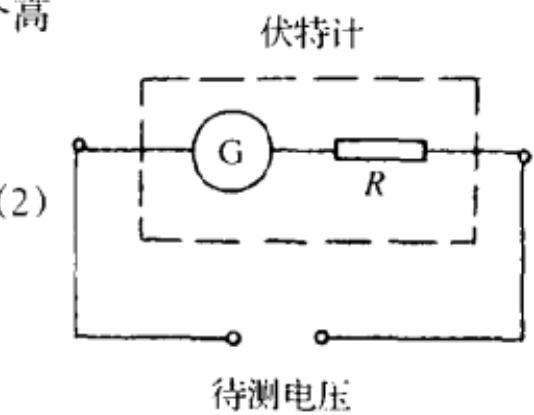
\includegraphics[width=0.5\linewidth]{figures/fig_4_2_7.jpg}
\end{center}

\vfill

\textbf{4.2.8.} 有一个内阻为 $R_{g}$ 的电流计，能通过的最大电流为 $I_{g}$ ，因此它能测量的最高电压为 $U_{g} = I_{g}R_{g}$ . 现在要将它改装成量程为 $U = nU_{g}$ 的伏特计 $(n > 1)$ ，试

问应如何办?用它测量电压时如何接法?试画出电路图.

图4.2.8

【解答】本题要求:这电流计通过电流 $I_{g}$ (即它两端的电压为 $U_{g}=I_{g}R_{g}$ ) 时, 被测量的电压为 $U=nU_{g}$ . 故必须将多余的电压 $(n-1)U_{g}=(n-1)I_{g}R_{g}$ 安排在它外边. 因此, 要与它串联一个电阻 R, 使得

$$
\begin{array}{r l} I _ {g} R & = (n - 1) U _ {g} = (n - 1) I _ {g} R _ {g} \\ & R = (n - 1) R _ {g} \end{array}\tag{所以}
$$

用它测量电压时,接法如图 4.2.8 所示.
\begin{center}
    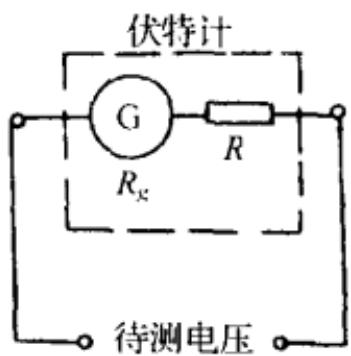
\includegraphics[width=0.5\linewidth]{figures/fig_4_2_8.jpg}
\end{center}

\vfill

\newpage

\textbf{4.2.9.} 有一个内阻为 $R_{g}$ 的电流计，它的量程为 $I_{g}$ . (1) 现在要把它的量程扩大为 $I = nI_{g}, n > 1$ ，问应如何办？用它测量电流时如何接法？试画出电路图. (2) 当 $R_{g} = 50\Omega, I_{g} = 2.0\mathrm{mA}, I = 0.50\mathrm{A}$ 时，试算出具体数据.

【解答】(1)这电流计能通过的最大电流为 $I_g$ ，现在要使它通过的电流为 $I_g$ 时，被测量的电流为 $nI_{g}$ . 故必须使多余的电流 $(n - 1)I_{g}$ 从它外边流过. 因此, 要与它并联一个电阻 $R$ , 使得

图4.2.9

$$
\begin{array}{r l} (n - 1) I _ {g} R & = I _ {g} R _ {g} \\ R & = \frac {R _ {g}}{n - 1} \end{array}
$$

用它测量电流时, 将它和 R 并联后两端 a、b 接到待测电路中, 如图 4.2.9 所示.

(2) 当 $R_{\mathrm{g}} = 50\Omega, I_{\mathrm{g}} = 2.0\mathrm{mA}, I = 0.50\mathrm{A}$ 时， $n = \frac{0.50}{2.0\times 10^{-3}} = 250$ ，故得

$$
R = \frac {5 0}{2 5 0 - 1} = 0. 2 0 (\Omega)
$$
\begin{center}
    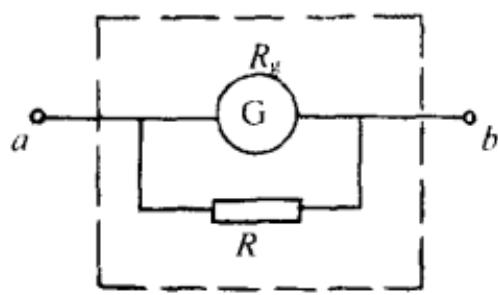
\includegraphics[width=0.5\linewidth]{figures/fig_4_2_9.jpg}
\end{center}

\vfill

\textbf{4.2.10.} 一电流计 G 的电阻为 $R_{g}=25\Omega$ ，指针偏转满格时，流过它的电流为 10mA。现在将它改装成 0.10A、1.0A 和 10A 三个量程的安培计，线路接法如图 4.2.10(1) 所示。试求电阻 $R_{1}$ 、 $R_{2}$ 和 $R_{3}$ 的值。

图 4.2.10(1)

图4.2.10(2)
\begin{center}
    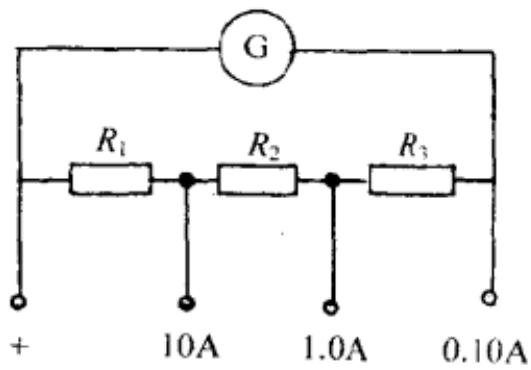
\includegraphics[width=0.5\linewidth]{figures/fig_4_2_10_1.jpg}
\end{center}
\begin{center}
    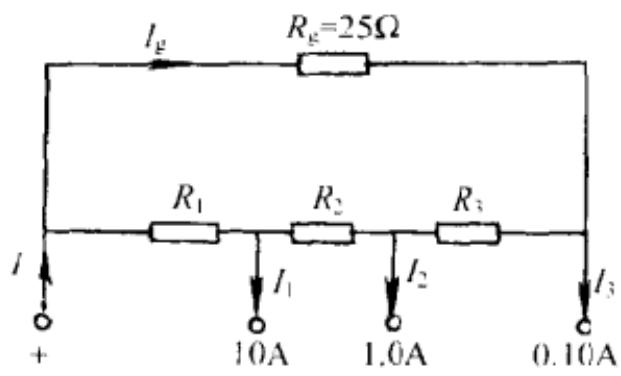
\includegraphics[width=0.5\linewidth]{figures/fig_4_2_10_2.jpg}
\end{center}

\vfill

\newpage

\textbf{4.2.11.} 一个三量程的伏特计内部线路如图 4.2.11 所示, 其中 $R_{g}=15.0\Omega$ 是转动线圈的电阻; 当指针偏转满格时, 通过 $R_{g}$ 的电流为 1.00mA. 试求电阻 $R_{1}$ 、 $R_{2}$ 和 $R_{3}$ 的值以及每个量程的电阻.

图4.2.11
\begin{center}
    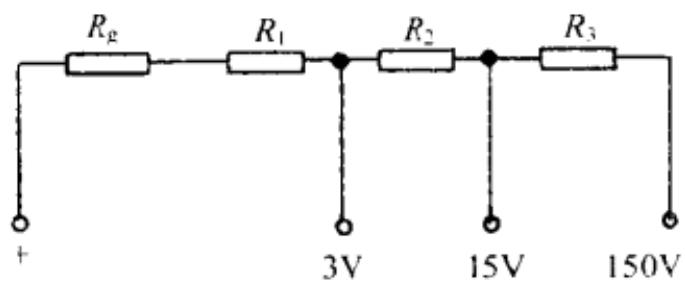
\includegraphics[width=0.5\linewidth]{figures/fig_4_2_11.jpg}
\end{center}

\vfill

\textbf{4.2.12.} 一伏特计有三个量程,分别为 1.5V、3.0V 和 15V,其中 15V 量程的电阻为 1500Ω.(1)试问其他两个量程的电阻各为多少?(2)将这伏特计接到一电池的两极,当用 1.5V 量程时,读数为 1.42V;若改用 3.0V 量程时,读数为 1.48V.两个读数为什么不同?用哪个较好?并计算这个电池的电动势和内阻的值.

\vfill

\newpage

\textbf{4.2.13.} 有三个伏特计 A、B 和 C，它们的量程都相同，但电阻各不相同， $R_{A}=1200\Omega, R_{B}=800\Omega, R_{C}=a$ $1000\Omega$ . 当它们联接如图 4.2.13 后，在 a、b 两端加上电压 U，A 的读数为 4.80V，C 的读数为 10.0V. 如果三者串联后再加电压 U，试问每个伏特计的读数各是多少？

图4.2.13
\begin{center}
    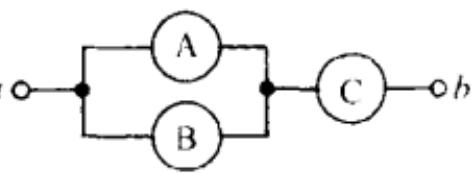
\includegraphics[width=0.5\linewidth]{figures/fig_4_2_13.jpg}
\end{center}

\vfill

\textbf{4.2.14.} 一段电路如图 4.2.14, 其中 $\varepsilon = 3.0V, r = 2.0\Omega, R = 8.0\Omega, I = 1.0A$ . 试问: (1) $a^{a}$ 点的电势比 b 点的高多少? (2) 电源作功的功率是多少? (3) 电源输出的功率是多少? (4) 若电流反


$$
\begin{array}{r l} \text {【解】} & (1) U _ {a} - U _ {b} = - I R + \mathcal {E} - I r = - 1. 0 \times 8. 0 + 3. 0 - 1. 0 \times 2. 0 \\ & = - 7. 0 (\mathrm{V}) \end{array}
$$

负号表示，a 点的电势比 b 点的低。

(2)电源作功(电源中非静电力作功)的功率为

$$
P = I \mathcal {E} = 1. 0 \times 3. 0 = 3. 0 (\mathrm{W})
$$

(3)电源输出的功率为

$$
P _ {0} = I U = I \mathcal {E} - I ^ {2} r = 3. 0 - 1. 0 ^ {2} \times 2. 0 = 1. 0 (\mathrm{W})
$$

(4) 若电流 I 反向, 则

$$
U _ {a} ^ {\prime} - U _ {b} ^ {\prime} = I R + \varepsilon + I r = 1. 0 \times 8. 0 + 3. 0 + 1. 0 \times 2. 0 = 1 3. 0 (\mathrm{V})
$$

这时 a 点的电势比 b 点的高. 电源做功的功率为

$$
P ^ {\prime} = - I \varepsilon = - 1. 0 \times 3. 0 = - 3. 0 (\mathrm{W})
$$

负号表示电源(电源中非静电力)作负功,这时电源充电,外界对电源作正功.电源输出的功率为

$$
P _ {0} ^ {\prime} = - I U = - I (\mathcal {E} + I r) = - 1. 0 \times (3. 0 + 1. 0 \times 2. 0) = - 5. 0 (\mathrm{W})
$$

负号表示,外界输入电源的功率为5.0W.其中3.0W储存在电源中,2.0W则消耗在r的焦耳热上.
\begin{center}
    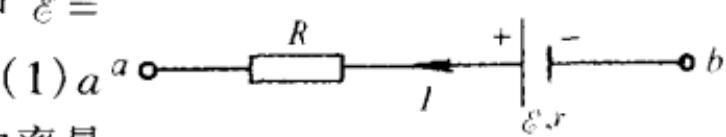
\includegraphics[width=0.5\linewidth]{figures/fig_4_2_14.jpg}
\end{center}

\vfill

\newpage

\textbf{4.2.15.} 一部分电路如图 4.2.15 所示, 其中 $\varepsilon = 2.0$ 伏, $r = 2.0\Omega$ , $R_{1} = 8.0\Omega$ , $R_{2} = 6.0\Omega$ , $I_{1} = 1.0A$ , $I_{2} = 0.5A$ . 试求 a、b 两端的电势差 $U_{ab}$ .

图4.2.15
\begin{center}
    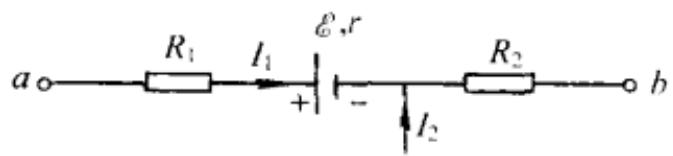
\includegraphics[width=0.5\linewidth]{figures/fig_4_2_15.jpg}
\end{center}

\vfill

\textbf{4.2.16.} 一电路如图 4.2.16 所示, 以地的电势为零, 试分别求 a、b 两点的电势.

\vfill

\newpage

\textbf{4.2.17.} 两个电池的电动势都是 $\mathcal{E}$ , 内阻分别为 $r_1$ 和 $r_2$ , 将它们串联后接到电阻 $R$ 上, 如图 4.2.17 所示. (1) 试问 $R$ 为什么值时, 内阻为 $r_1$ 的电池的端电压为零? (2) 这时该电池还起作用吗?

\vfill

\textbf{4.2.18.} 一电路如图 4.2.18 所示, 其中 $\varepsilon_{1}, r_{1}, \varepsilon_{2}, r_{2}$ 和 R 都已知. 试求通过 R 的电流 I.

\vfill

\newpage

\textbf{4.2.19.} 三个电池并联如图 4.2.19(1)，已知 $\varepsilon_{1}=1.40V,\varepsilon_{2}=1.50V,\varepsilon_{3}=1.80V,r_{1}=r_{2}=1.00\Omega,r_{3}=1.60\Omega$ . 试求每个电池的电流、端电压和输出功率.

图4.2.19(1)
图 4.2.19(2)
\begin{center}
    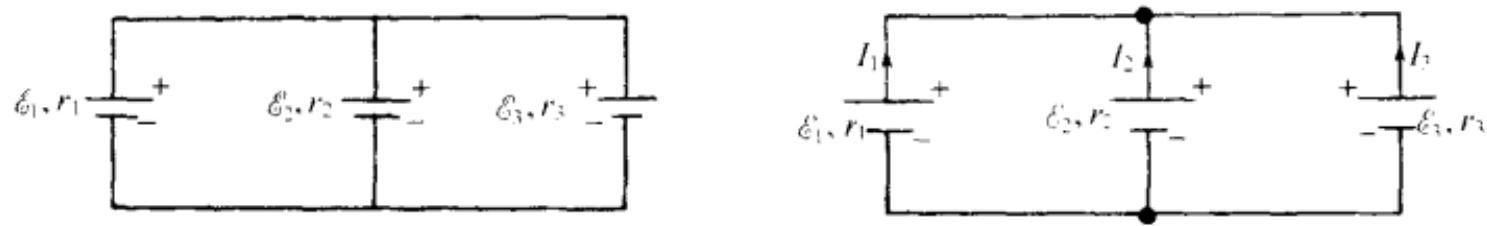
\includegraphics[width=0.5\linewidth]{figures/fig_4_2_19.jpg}
\end{center}

\vfill

\textbf{4.2.20.} 一电路如图 4.2.20 所示, 已知其中 $\varepsilon_{1} = 12.0$ 伏, $\varepsilon_{2} = \varepsilon_{3} = 6.0\mathrm{V}, R_{1} = R_{2} = R_{3} = 3.0\Omega$ , 电源的内阻都可略去不计. 试分别求 $a, b$ 两点的电势差 $U_{ab}$ , $a, c$ 两点的电势差 $U_{ac}$ 以及 $b, c$ 两点的电势差 $U_{bc}$ .

\vfill

\newpage

\textbf{4.2.21.} 图 4.2.21 是一个三极管的电路, 其中电流 I 从板极 A 到阴极 K; 从板极 A 到栅极 G 的电流可略去不计. 已知 $I = 10 \, mA, R_{3} = 10 \, k\Omega, \varepsilon = 300 \, V, \varepsilon$ 的内阻可略去不计. (1) 以地的电势为零, 试分别求 A 和 G 的电势 $U_{A}$ 和 $U_{G}$ ; (2) 若 $U_{G} - U_{K} = -15 \, V$ , 试求 $R_{2}$ 以及 $U_{AK} = U_{A} - U_{K}$ .

\vfill

\textbf{4.2.22.} 一电路如图 4.2.22, 其中 $\varepsilon_{1}=1.5V, \varepsilon_{2}=1.0V$ , 电源的内阻都可略去不计. 试求 $R_{3}$ 中的电流为零时, $R_{1}$ 与 $R_{2}$ 的比值 $R_{1}/R_{2}$ .

\vfill

\newpage

\textbf{4.2.23.} 电势差计(电位计)是准确测量电势差的仪器,它的线路如图4.2.23所示,其中 $\varepsilon$ 是辅助电源的电动势,其内阻可略去不计; $\varepsilon_{x}$ 是待测电源(或标准电源)的电动势,其内阻为r(图中画在电源外);R是一个均匀电阻(在它上面各处,单位长度的电阻都相同),它的长度为ab=l,c是它上面的一个滑动接头,a到c的长度为ac=x.设 $\varepsilon_{x}\varepsilon_{x}$ 和l都已知.(1)试求电势差计平衡(即通过 $\varepsilon_{x}$ 的电流为零)时x的值 $x_{0}$ ;(2)当 $x\neq x_{0}$ 时,通过 $\varepsilon_{x}$ 的电流方向如何?(3)若 $\varepsilon<\varepsilon_{x}$ ,结果如何?

图4.2.23
\begin{center}
    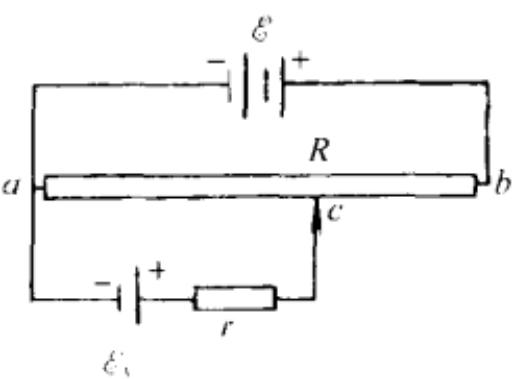
\includegraphics[width=0.5\linewidth]{figures/fig_4_2_23.jpg}
\end{center}

\vfill

\textbf{4.2.24.} 一电路如图4.2.24所示，其中 $\varepsilon_{1},\varepsilon_{2}$ 和 $R_{1},R_{2},R_{3}$ 都已知，电源的内阻已分算入 $R_{1}$ 和 $R_{2}$ 内，试求电流 $I_{1},I_{2}$ 和 $I_{3}$

\vfill

\newpage

\textbf{4.2.25.} 电路如图 4.2.25 所示, 其中 $\varepsilon_{1}=12.0V, \varepsilon_{2}=6.0V, r_{1}=r_{2}=R_{1}=R_{2}=1.0\Omega$ , 通过 $R_{3}$ 的电流为 $I_{3}=3.0A$ , 流向如图所示. 试求通过 $R_{1}$ 的电流 $I_{1}$ 和通过 $R_{2}$ 的电流 $I_{2}$ 以及 $R_{3}$ 的值.

\vfill

\textbf{4.2.26.} 一电路如图 4.2.26 所示, 其中 $\varepsilon_{1}=1.5V, \varepsilon_{2}=1.0V, R_{1}=50\Omega, R_{2}=80\Omega, R=10\Omega$ , 电源的内阻都可略去不计, 试求通过 R 的电流 I.
\begin{center}
    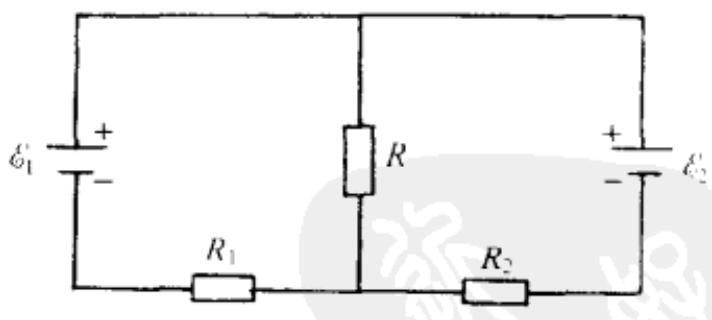
\includegraphics[width=0.5\linewidth]{figures/fig_4_2_26.jpg}
\end{center}

\vfill

\newpage

\textbf{4.2.27.} 一电路如图 4.2.27(1)，其中 $\varepsilon_{1}=3.0V,\varepsilon_{2}=1.5V,\varepsilon_{3}=2.2V,R_{1}=1.5\Omega,R_{2}=2.0\Omega,R_{3}=1.4\Omega$ ，电源的内阻都已分别算在 $R_{1}$ 、 $R_{2}$ 和 $R_{3}$ 内，试求 a、b 两点的电势差 $U_{ab}$ .

图 4.2.27(1)

图4.2.27(2)
\begin{center}
    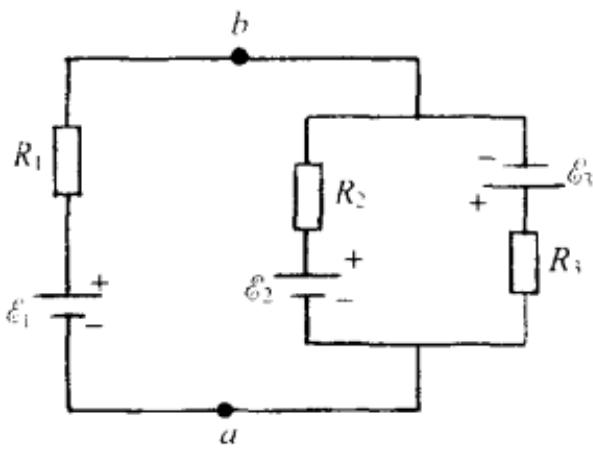
\includegraphics[width=0.5\linewidth]{figures/fig_4_2_27_1.jpg}
\end{center}
\begin{center}
    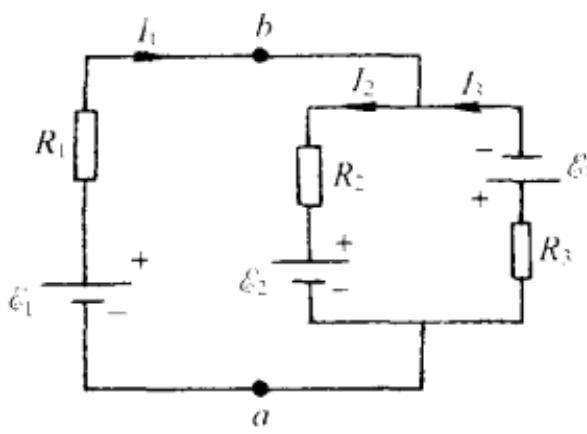
\includegraphics[width=0.5\linewidth]{figures/fig_4_2_27_2.jpg}
\end{center}

\vfill

\textbf{4.2.28.} 一电路如图 4.2.28, 其中 $\varepsilon_{1}=12.0V, \varepsilon_{2}=10.0V, \varepsilon_{3}=8.0V, r_{1}=r_{2}=r_{3}=1.0\Omega, R_{1}=R_{3}=R_{4}=R_{5}=2.0\Omega, R_{2}=3.0\Omega$ . 试求: (1) a、b 断开时的 $U_{ab}$ ; (2) a、b 短路时通过 $\varepsilon_{1}$ 的电流的大小和方向.

\vfill

\newpage

\textbf{4.2.29.} 一电路如图4.2.29(1)所示,其中 $\varepsilon_{1}=1.0V,\varepsilon_{2}=2.0V,\varepsilon_{3}=3.0V,r_{1}=r_{2}=r_{3}=R_{1}=1.0\Omega,R_{2}=3.0\Omega$ .试求:(1)通过 $\varepsilon_{3}$ 的电流;(2) $R_{2}$ 消耗的功率;(3) $\varepsilon_{3}$ 输出的功率.

\vfill

\textbf{4.2.30.} 一电路如图 4.2.30 所示, 试求其中的 $\varepsilon_{1}, \varepsilon_{2}$ 和 $U_{ab}$ .

\vfill

\newpage

\textbf{4.2.31.} 一电路如图 4.2.31 所示, 已知 $\varepsilon_{1}=6.0V, \varepsilon_{2}=12.0V$ , 它们的内阻都可略去不计; $6\Omega$ 电阻中的电流为 I=1.0A, 方向如图所示. (1) 试求通过 X 的电流 $I_{x}$ ; (2) X 是什么?

\vfill

\textbf{4.2.32.} 甲乙两站相距 $50\mathrm{km}$ , 其间有两条相同的电话线, 有一条因在某处触地而发生故障, 甲站的检修人员用图 4.2.32 的办法找出触地处到甲站的距离 $x$ . 让乙站把电话线两端短路 (即接在一起), 作为电桥的一臂, 调节 $r$ 使通过检流计 $G$ 的电流为零, 已知电话线每公里长的电阻为 $6.0\Omega$ , 测得 $r = 360\Omega$ . 试求 $x$ .

图4.2.32
\begin{center}
    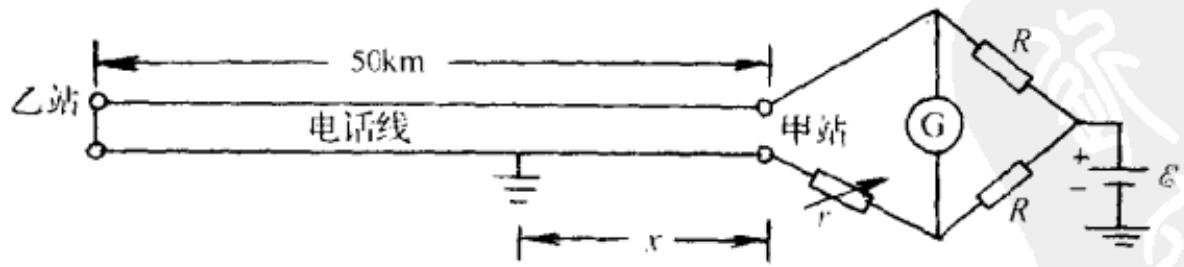
\includegraphics[width=0.5\linewidth]{figures/fig_4_2_32.jpg}
\end{center}

\vfill

\newpage

\textbf{4.2.33.} 为了找出电缆在某处由于损坏而触地, 可以使用图 4.2.33 的装置. AB 是一条长为 100cm 的电阻线, 接头 C 可以在它上面滑动. 已知电缆长 7.8km, 设当 C 滑到 $\overline{CB} = 41cm$ 时, 通过电流计 G 的电流为零. 试求电缆损坏处到 B 的距离.

图4.2.33
\begin{center}
    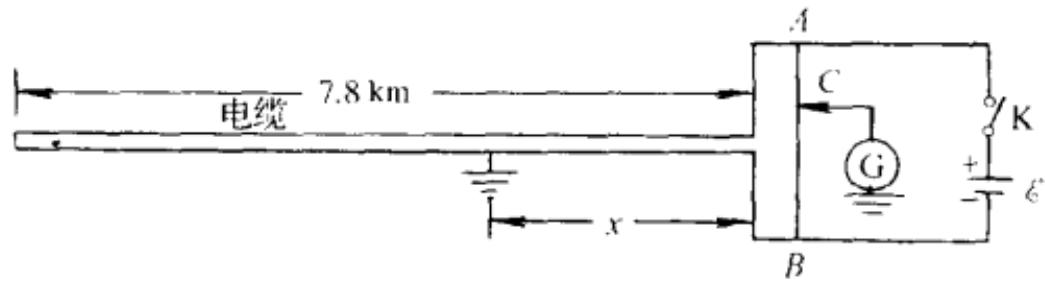
\includegraphics[width=0.5\linewidth]{figures/fig_4_2_33.jpg}
\end{center}

\vfill

\textbf{4.2.34.} 一电缆 $AB$ 长 $50\mathrm{km}$ , 中间某处发生障碍(即漏电). 现在作如下检查(图B4.2.34): 将 $B$ 端断开, 在 $A$ 端加上 $200\mathrm{V}$ 电压, 测得 $B$ 端电压为 $40\mathrm{V}$ ; 再将 $A$ 端断开, 在 $B$ 端加上可调的电压, 当调到 $300\mathrm{V}$ 时, $A$ 端电压为 $40\mathrm{V}$ . 试求发生障碍处到 $A$ 端

的距离 $x$

\vfill

\newpage

\textbf{4.2.35.} 惠斯通电桥的电路如图 4.2.35(1) 所示, 设其中电阻 $R_{1}$ 、 $R_{2}$ 、 $R_{3}$ 、 $R_{4}$ 和 $R_{g}$ 以及电源的电动势 $\varepsilon$ 和它的内阻 $r$ 都已知. (1) 试求通过 $R_{g}$ 的电流 $I_{g}$ ; (2) 在什么情况下, $I_{g}$ 是从 $C$ 到 $D$ ? 在什么情况下, $I_{g}$ 是从 $D$ 到 $C$ ?

图4.2.35(1)

图4.2.35(2)
\begin{center}
    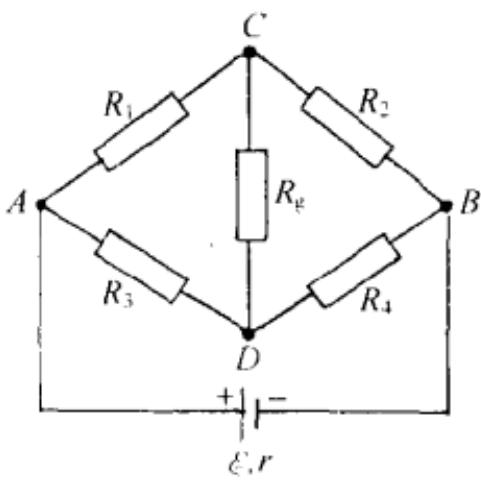
\includegraphics[width=0.5\linewidth]{figures/fig_4_2_35_1.jpg}
\end{center}
\begin{center}
    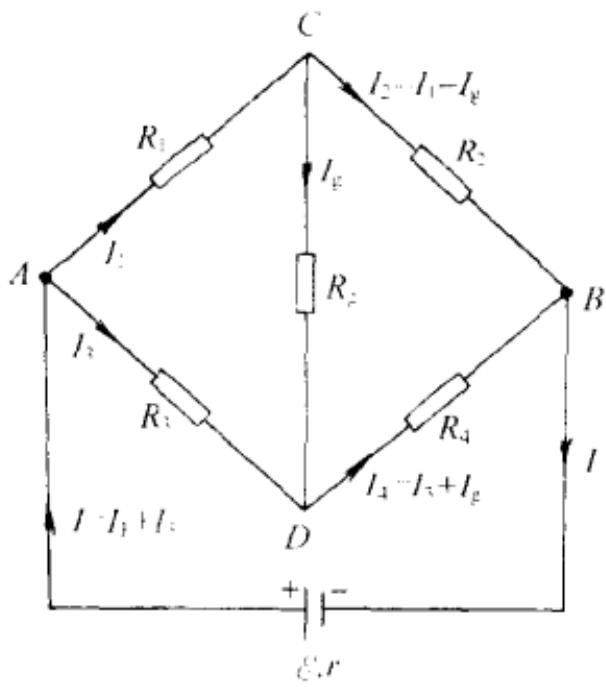
\includegraphics[width=0.5\linewidth]{figures/fig_4_2_35_2.jpg}
\end{center}

\vfill

\textbf{4.2.36.} 有了基尔霍夫定律,任何复杂的稳恒直流电路,在原则上都可以解决;但在实际问题里,直接用基尔霍夫定律解题往往很繁复.一些特定的问题,用某种特定的规律或方法求解,有时比较简便,戴维南(Thévenin)定理就是这种规律之一.戴维南定理(有的书上称为等效电源定理)如下:在任何复杂的稳恒直流电路里,任何一个电阻 R [图 4.2.36(1)]中流过的电流 i 都可以用下式表示:

图4.2.36(1)

图4.2.36(2)

$$
i = \frac {u}{R + r}
$$

式中 u 是把 R 断开(也就是令 $R = \infty$ ) 时, a、b 之间的电压; r 是把 R 断开并且使电路中所有电源的电动势都为零时, a、b 之间的电阻. 试用戴维南定理求前面 4.2.35 题惠斯通电桥里通过检流计 $R_{g}$ 的电流 $I_{g}$ .
\begin{center}
    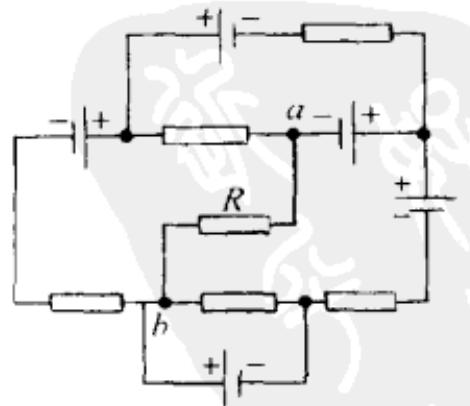
\includegraphics[width=0.5\linewidth]{figures/fig_4_2_36_1.jpg}
\end{center}
\begin{center}
    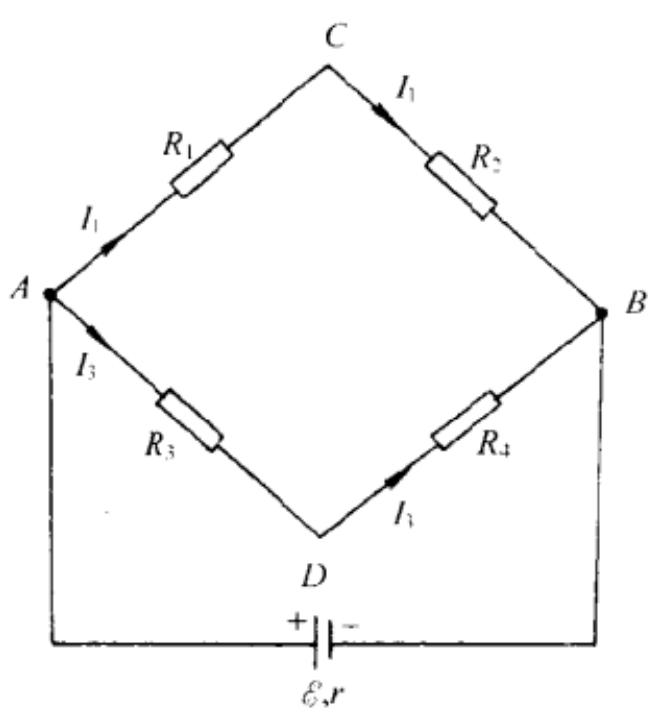
\includegraphics[width=0.5\linewidth]{figures/fig_4_2_36_2.jpg}
\end{center}

\vfill

\newpage

\textbf{4.2.37.} 六个相同的电阻 $r = 1.0\Omega$ ，联接成如图4.2.37所示的电路。在 a、b 间加上 U = 10V 的电势差，试求每个电阻中的电流。

\vfill

\textbf{4.2.38.} (1)如图4.2.38(1)中， $a, b$ 间的电阻为 $R$ ，试问(i) $R$ 短路（如用导线把 $R$ 两端接在一起）和(ii) $R$ 开路（如 $R$ 断开）时， $a, b$ 间的电阻各是多少？(2)如图4.2.38(2)中， $a, b$ 间的电容为 $C$ ，试问(i) $C$ 短路（如用导线把 $C$ 的两极板接在一起）和(ii) $C$ 开路（如 $C$ 断开）时， $a, b$ 间的电容各是多少？(3)在一电路中，如 $a, b$ 两点间短路，从电阻的角度看， $R$ 为零，从电容的角度看， $C$ 为 $\infty$ ；如 $a, b$ 两点间开路，从电阻的角度看， $R$ 为 $\infty$ ，从电容的角度看， $C$ 为零。你认为对吗？试略加说明。

(i)
(ii)

(2)
图4.2.38

【解答】（1）(i) $R_{ab}=0$ ; (ii) $R_{ab}=\infty$ .

(2)(i) $C_{ab}=\infty$ ; (ii) $C_{ab}=0$ .

(3) 对. $a, b$ 间短路: 在 $a, b$ 间加上电压, 便有非常大的电流流过, 故从电阻的角度看, $a, b$ 间的电阻非常小, 可看作零; 从电容的角度看, 电流不断地流, 相当于 $a, b$ 间有一个电容为无穷大的电容器.

a、b间开路：在a、b间加上电压，电流为零.从电阻的角度看，a、b间的电阻为无穷大；从电

容的角度看,电荷不能流入,相当于a、b间有一个电容为零的电容器.
\begin{center}
    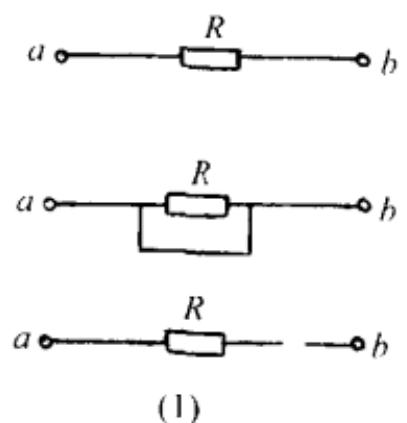
\includegraphics[width=0.5\linewidth]{figures/fig_4_2_38_1.jpg}
\end{center}
\begin{center}
    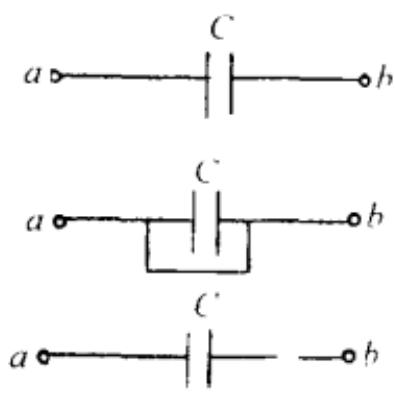
\includegraphics[width=0.5\linewidth]{figures/fig_4_2_38_2.jpg}
\end{center}

\vfill

\newpage

\textbf{4.2.39.} 一平行板电容器两极板间充满电阻率为 $\rho$ 、电容率为 $\varepsilon$ 的均匀介质，因而两极板间的电阻为 $R$ （漏电电阻）。（1）设这电容器的电容为 $C$ ，试证明： $RC = \varepsilon \rho$ ；（2）这电容器充电后，去掉电源，两极板间的电势差便逐渐减小，试证明：电势差下降的速率由介质的特性 $\varepsilon$ 和 $\rho$ 决定，而与电容的大小和电容器的形状无关。

\vfill

\textbf{4.2.40.} 丹聂耳电池由两个同轴圆筒构成, 长为 l, 外筒是内半径为 b 的铜, 内筒是外半径为 a 的锌, 两筒间是电容率为 $\varepsilon$ 、电阻率为 $\rho$ 的硫酸铜溶液, 如图 4.2.40 所示. 略去边缘效应. 试求: (1) 这电池的内阻 R; (2) 两筒之间的电容 C; (3) R 与 C 之间的关系.

\vfill

\newpage

\textbf{4.2.41.} 一平行板电容器两极板的面积均为 S，两板间充满两层均匀介质，它们的厚度分别为 $d_{1}$ 和 $d_{2}$ ，电容率分别为 $\varepsilon_{1}$ 和 $\varepsilon_{2}$ ，电导率分别为 $\sigma_{1}$ 和 $\sigma_{2}$ ，如图4.2.41所示。当两极板的电势差为 $U$ 时，略去边缘效应，试求：(1)两介质中的电场强度和电位移；(2)两介质交界面上电荷量的面密度；(3)通过这电容器的电流；(4) $\sigma_{1} = 0$ 的情况。

图4.2.41
\begin{center}
    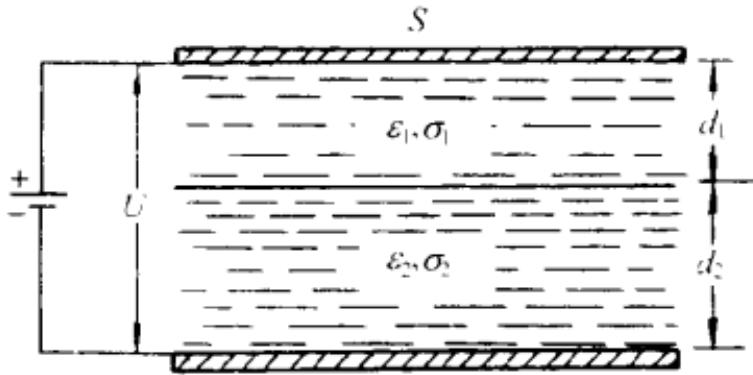
\includegraphics[width=0.5\linewidth]{figures/fig_4_2_41.jpg}
\end{center}

\vfill

\textbf{4.2.42.} 导线里的电流 I 既然有方向,为什么不是矢量?

【解答】电流(电流强度) $I$ 是单位时间内通过给定面积的电荷量, 它只有正负 (如规定正电荷从该面积的一边流到另一边为正, 反过来便为负), 而无方向. 通常说的导线里的 $I$ 的方向, 实际上是指它的值的正负.

描述电荷在空间流动状态的量是电流密度 j，它是矢量。电流(电流强度) I 与电流密度 j 的关系为

$$
I = \iint_ {S} \boldsymbol {j} \cdot \mathrm{d} \boldsymbol {S}
$$

式中积分是对某个面积 S 的积分. 由此亦可见 I 不是矢量.

\vfill

\newpage

\textbf{4.2.43.} 一铜线直径为 $1.0\mathrm{cm}$ , 载有 $200\mathrm{A}$ 的电流, 已知铜的电阻率为 $\rho = 1.72 \times 10^{-8} \Omega \cdot \mathrm{m}$ , 试求这铜线里电场强度的大小 $E$ . 这铜线上相距 $100\mathrm{m}$ 的两点电势差是多少?

\vfill

\textbf{4.2.44.} 在曲面上有一层面电流, 面电流密度为 k, 在这曲面上有一段曲线 ab [图 4.2.44(1)], 试证明: 通过这段曲线的电流为 $I = \int_{a}^{b} k \cdot (\mathrm{d}l \times n)$ , 式中 dl 是 ab 曲线上的线元, 其方向如图 4.2.44 所示, n 是该曲面在 dl 处法线方向上的单位矢量.

\vfill

\newpage

\textbf{4.2.45.} 一个很小的放射源,每秒钟放射出 N 个带电粒子,每个粒子所带的电荷量为 q;设放射是各向同性的,试求离这放射源为 r 处的电流密度 j.

图4.2.44(2)

\vfill

\textbf{4.2.46.} 电荷量 Q 均匀地分布在半径为 R 的球体内, 这球以匀角速度 $\omega$ 弧度/秒绕它的一个固定的直径旋转. 试求球内离转轴为 r 处的电流密度 j.

图4.2.46
\begin{center}
    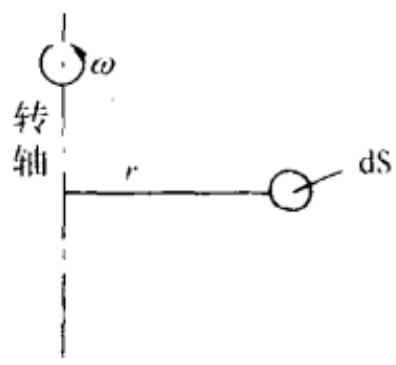
\includegraphics[width=0.5\linewidth]{figures/fig_4_2_46.jpg}
\end{center}

\vfill

\newpage

\textbf{4.2.47.} 一镍铬合金丝的横截面积为 $0.20\mathrm{mm}^2$ ，电阻率为 $1.0\times 10^{-6}\Omega \cdot \mathrm{m}$ 现在用它作电炉的电阻丝，在它两端加上120伏的直流电压，发热的功率为600W，试问它的长度应为多少？

\vfill

\textbf{4.2.48.} 有两个电灯泡,分别标明 110V 40W 和 110V 120W,如果把它们串联起来接到 220 伏的电源上,其中一个马上就烧坏了.哪个灯泡烧坏了?为什么会烧坏?如果两个灯泡都是 110V 40W 的,则如何?

【解答】110V 40W 灯泡的电阻和额定电流分别为

$$
R _ {1} = \frac {U _ {1} ^ {2}}{P _ {1}} = \frac {1 1 0 ^ {2}}{4 0} = 3 0 3 (\Omega)
$$

$$
I _ {1} = \frac {P _ {1}}{U _ {1}} = \frac {4 0}{1 1 0} = 0. 3 6 4 (\mathrm{A})
$$

110V 120W 灯泡的电阻和额定电流分别为

$$
R _ {2} = \frac {U _ {2} ^ {2}}{P _ {2}} = \frac {1 1 0 ^ {2}}{1 2 0} = 1 0 1 (\Omega)
$$

$$
I _ {2} = \frac {P _ {2}}{U _ {2}} = \frac {1 2 0}{1 1 0} = 1. 0 9 (\mathrm{A})
$$

两灯泡串联后，总电阻为

$$
R = R _ {1} + R _ {2} = 3 0 3 + 1 0 1 = 4 0 4 (\Omega)
$$

接到 220V 的电压上,通过的电流为

$$
I = \frac {U}{R} = \frac {2 2 0}{4 0 4} = 0. 5 4 5 (\mathrm{A})
$$

因 I 超出 $I_{1}$ 很多, 故烧坏的是 110V 40W 的灯泡. 烧坏的原因是通过的电流太大, 发热过多, 使灯泡的灯丝熔化而断裂.

如果两个灯泡都是 110V 40W 的,串联后接到 220V 的电源上,则加在每个灯泡上的电压便都是 110V,就能正常发光而不会烧坏.

\vfill

\newpage

\textbf{4.2.49.} 在一升 $0^{\circ}$ C 的水里有一个 $R = 20\Omega$ 的电阻, 现在 R 两端加上 100V 的电压, 试问经过多长时间水热到 $100^{\circ}$ C? 此后如继续加热 10min, 有多少克的水化为蒸汽? 已知水的汽化热为 539cal/g. 假定电阻发的热全部用于升高水温或使水汽化, 且电阻随温度的变化可略去不计.

\vfill

\textbf{4.2.50.} 蓄电池充电的电路如图4.2.50所示,其中R是可变电阻,L是规格为6V 3W的指示灯,V是伏特计.接通开关K,当R调到20Ω时,指示灯正常发光,伏特计的读数为52V.已知蓄电池的内阻为2.0Ω;伏特计消耗的功率很小,可略去不计.试求:(1)充电

图4.2.50

机输出的功率；(2)输入蓄电池的功率；(3)转化为蓄电池中化学能的功率.
\begin{center}
    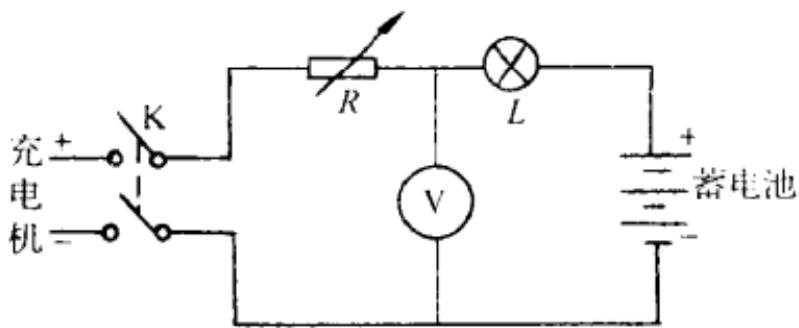
\includegraphics[width=0.5\linewidth]{figures/fig_4_2_50.jpg}
\end{center}

\vfill

\newpage

\textbf{4.2.51.} 在电源输出功率时,有时要考虑效率问题.如图 4.2.51,电源的电动势为 $\varepsilon$ , 内阻为 r, 负载的电阻为 R.试证明: 当 R = r 时, 电源的输出功率达到最大; 最大功率的值为 $P_{\max} = \frac{\varepsilon^{2}}{4R}$ .

\vfill

\textbf{4.2.52.} 有一个标明 $1\mathrm{k}\Omega$ 40W 的电位器, 试问: (1) 允许通过它的最大电流是多少? (2) 允许加在它两端的最高电压是多少? (3) 在它两端加上 $10\mathrm{V}$ 电压时, 它消耗的功率是多少?

【解答】(1)允许通过它的最大电流为

$$
I _ {\mathrm{mex}} = \sqrt {\frac {P}{R}} = \sqrt {\frac {4 0}{1 0 ^ {3}}} = 0. 2 (\mathrm{A})
$$

(2)允许加在它两端的最高电压为

$$
U _ {\max} = \frac {P}{I} - \frac {4 0}{0 . 2} = 2 0 0 (\mathrm{V})
$$

(3)消耗的功率为

$$
P = \frac {U ^ {2}}{R} = \frac {1 0 ^ {2}}{1 0 ^ {3}} = 0. 1 (\mathrm{W})
$$

\vfill

\newpage

\textbf{4.2.53.} 一并激直流电动机的电路如图4.2.53所示，外加电压为 $120\mathrm{V}$ ，它的励磁绕组的电阻为 $R = 240\Omega$ ，电枢电阻为 $r = 3\Omega$ 。电动机运转时，电枢中产生反电动势 $\mathcal{E}$ ，其方向与加到电枢上的外电压方向相反。电动机由外面取得的电流为 $I = 4.5\mathrm{A}$ 。试求：(1)励磁电流 $i_R$ ；(2)电枢电流 $i$ ；(3)反电动势 $\mathcal{E}$ ；(4)励磁绕组因发热而消耗的功率 $P_R$ ；(5)电枢因发热而消耗的功率 $P_r$ ；(6)外面输入这电动机的功率 $P_i$ ；(7)这电动机的效率 $\eta$ （已知由于机械摩擦等损耗的功率为 $P_\mu = 50\mathrm{W}$ ）。

\vfill

\textbf{4.2.54.} 试证明:电流在导电物体中流过时,该物体单位体积内产生的焦耳热为 $E^{2}/\rho = \rho j^{2} = j \cdot E$ , 式中 $\rho$ 为该物体的电阻率, E 为电场强度, j 为电流密度.
\begin{center}
    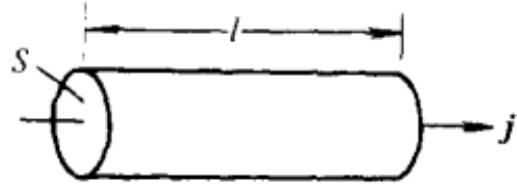
\includegraphics[width=0.5\linewidth]{figures/fig_4_2_54.jpg}
\end{center}

\vfill

\newpage

\textbf{4.2.55.} 试证明:一定的电流 I 在流经 $R_{1}$ 和 $R_{2}$ 并联的电路时,电流在这两条支路里是这样分布的, $R_{1}$ 和 $R_{2}$ 消耗的焦耳热之和为最小.
\begin{center}
    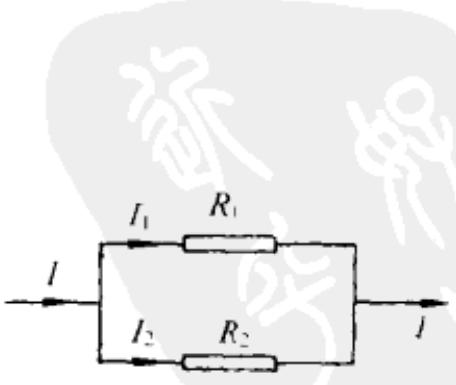
\includegraphics[width=0.5\linewidth]{figures/fig_4_2_55.jpg}
\end{center}

\vfill

\textbf{4.2.56.} 电学量的量纲可以用长度 L、质量 M、时间 T 和电流 I 四个基本量表示，如电荷 q 的量纲为 $[q] = TI$ 。试导出电场强度 E、电势 U、真空电容率 $\varepsilon_{0}$ 、电位移 D、电偶极矩 p、极化强度 P、电容 C 和电阻 R 的量纲。

$$
\text {   【解】   } \quad [ E ] = \left[ \frac {F}{q} \right] = \left[ \frac {m a}{q} \right] = \frac {\mathrm{MLT} ^ {- 2}}{\mathrm{TI}} = \mathrm{LMT} ^ {- 3} \mathrm{I} ^ {- 1}
$$

$$
[ U ] = [ \boldsymbol {E} \cdot \boldsymbol {l} ] = \mathrm{L} ^ {2} \mathrm{MT} ^ {- 3} \mathrm{I} ^ {- 1}
$$

$$
[ \varepsilon_ {0} ] = \frac {[ q ]}{[ r ^ {2} ] [ E ]} = \frac {\mathrm{TI}}{\mathrm{L} ^ {2} \cdot \mathrm{LMT} ^ {- 3} \mathrm{I} ^ {- 1}} = \mathrm{L} ^ {- 3} \mathrm{M} ^ {- 1} \mathrm{T} ^ {4} \mathrm{I} ^ {2}
$$

$$
[ \boldsymbol {D} ] = [ \varepsilon_ {0} \boldsymbol {E} ] = L ^ {- 3} M ^ {- 1} T ^ {4} I ^ {2} \cdot L M T ^ {- 3} I ^ {- 1} = L ^ {- 2} T I
$$

$$
[ \boldsymbol {p} ] = [ q l ] = \mathrm{TI} \cdot \mathrm{L} = \mathrm{LTI}
$$

$$
[ \boldsymbol {P} ] = \left[ \frac {\sum \boldsymbol {p}}{\Delta V} \right] = \frac {[ \boldsymbol {p} ]}{[ V ]} = \frac {\mathrm{LTI}}{\mathrm{L} ^ {3}} = \mathrm{L} ^ {- 2} \mathrm{TI}
$$

$$
[ C ] = \left[ \frac {q}{U} \right] = \frac {\mathrm{TI}}{\mathrm{L} ^ {2} \mathrm{MT} ^ {- 3} \mathrm{I} ^ {- 1}} = \mathrm{L} ^ {- 2} \mathrm{M} ^ {- 1} \mathrm{T} ^ {4} \mathrm{I} ^ {2}
$$

$$
[ R ] = \left[ \frac {U}{I} \right] = \frac {\mathrm{L} ^ {2} \mathrm{MT} ^ {- 3} \mathrm{I} ^ {- 1}}{\mathrm{I}} = \mathrm{L} ^ {2} \mathrm{MT} ^ {- 3} \mathrm{I} ^ {- 2}
$$

§ 4.3 电流的微观机制

\vfill

\newpage

\textbf{4.3.1.} 已知电子电荷量的大小为 $1.60 \times 10^{-19}C$ ，试问载有 1.00A 直流电流的导线，每秒钟有多少电子流过它的横截面？

\vfill

\textbf{4.3.2.} 一铜线直径为 $1.0\mathrm{cm}$ ，载有200A的电流。已知铜内自由电子的数密度为 $n = 8.5\times 10^{22}$ 个 $/ \mathrm{cm}^3$ ，每个电子电荷量的大小为 $1.6\times 10^{-19}\mathrm{C}$ ，试求这铜线中电子定向运动的平均速率 $\bar{u}$ 。

\vfill

\newpage

\textbf{4.3.3.} 一条铝线的横截面积为 $0.10\mathrm{mm}^2$ ，在室温 $300\mathrm{K}$ 时载有 $5.0\times 10^{-4}\mathrm{A}$ 的电流.设每个铝原子有三个电子参加导电.已知铝的原子量为27，室温下铝的密度为 $2.7\mathrm{g / cm}^3$ ，电阻率为 $2.8\times 10^{-8}\Omega \cdot \mathrm{m}$ ，电子电荷量的大小为 $1.6\times 10^{-19}\mathrm{C}$ ，电子质量 $m = 9.1\times 10^{-31}\mathrm{kg}$ ，阿伏伽德罗常量为 $6.0\times 10^{23}(\mathrm{mol})^{-1}$ ，玻耳兹曼常量 $k = 1.38\times 10^{-23}\mathrm{J / K}$ .试求这铝线内：(1)电子定向运动的平均速率 $\bar{u}$ ；(2)电子热运动的方均根速率 $\sqrt{v^2} = \sqrt{3kT / m}$ ；(3)电场强度的大小 $E$ ；(4)使 $\bar{u} = \sqrt{v^2}$ 所需的电场强度.

\vfill

\textbf{4.3.4.} 一铜棒的横截面积为 $20 \times 80\mathrm{mm}^2$ ，长为 $2.0\mathrm{m}$ ，两端的电势差为 $50\mathrm{mV}$ 。已知铜的电导率为 $\sigma = 5.7 \times 10^{7}\mathrm{S/m}$ ，铜内自由电子的电荷量密度为 $1.36 \times 10^{10}\mathrm{C/m}^{3}$ 。试求：(1)它的电阻 $R$ ；(2)电流 $I$ ；(3)电流密度的大小 $j$ ；(4)电场强度的大小 $E$ ；(5)所消耗的功率；(6)一小时所消耗的能量；(7)棒内电子定向运动的平均速率 $\bar{u}$ 。

\vfill

\newpage

\textbf{4.3.5.} 已知铜的原子量为 63.75, 密度为 $8.9 \mathrm{~g} / \mathrm{cm}^{3}$ ; 阿伏伽德罗常量 $N_{\mathrm{A}} = 6.022 \times 10^{23} (\mathrm{mol})^{-1}$ , 电子电荷量的大小为 $1.602 \times 10^{-19} \mathrm{C}$ , 铜导线里每个铜原子都有一个自由电子. 当铜导线里的电流密度 $j = 1.0 \mathrm{~A} / \mathrm{cm}^{2}$ 时, 试求电子沿铜线定向运动的平均速率 $\bar{u}$ . 既然铜内电子定向运动的平均速率这么小, 为什么电源一接通, 电路上各处便立刻都有电了?

\vfill

\textbf{4.3.6.} 已知铜的原子量为 63.75, 密度为 $8.9 \mathrm{~g} / \mathrm{cm}^{3}$ , 在铜导线里, 每个铜原子都有一个自由电子, 电子电荷量的大小为 $1.6 \times 10^{-19} \mathrm{C}$ , 阿伏伽德罗常量 $N_{\mathrm{A}} = 6.022 \times 10^{23} (\mathrm{~mol})^{-1}$ . (1) 技术上为了安全, 铜线内电流密度不得超过 $j_{\max} = 6.0 \mathrm{~A} / \mathrm{mm}^{2}$ , 试求电流密度为 $j_{\max}$ 时, 铜线内电子定向运动的平均速率 $\bar{u}_{\max}$ ; (2) 试按下列公式求 $T = 300 \mathrm{~K}$ 时铜线内电子热运动的平均速率: $\bar{v} = \sqrt{\frac{8 k T}{\pi m}}$ , 式中 $m = 9.11 \times 10^{-31} \mathrm{~kg}$ 是电子质量, $k = 1.38 \times 10^{23}$ 是玻尔兹曼常量, $T$ 是绝对温度; (3) $\bar{v}$ 是 $\bar{u}$ 的多少倍?

\vfill

\newpage

\textbf{4.3.7.} 在一真空二极管内，阴极和阳极是一对平行的导体片面积都是 $S = 2.0\mathrm{cm}^2$ ，它们之间的电流 $I$ ，完全由电子从阴极飞向阳极构成；当电流 $I = 50\mathrm{mA}$ 时，电子到达阳极时的速率是 $1.2\times 10^{7}\mathrm{m / s}$ .已知电子电荷量的大小为 $1.6\times 10^{-19}$ C.试求阳极表面外每立方毫米内的电子数.

\vfill

\textbf{4.3.8.} 电子管内阴极发射电子,阳极的电势比阴极高300伏,设电子从阴极出来时速度很小,可略去不计.已知电子质量为 $m=9.11\times10^{-31}$ kg,电子电荷量为 $e=-1.60\times10^{-19}$ C.(1)试求电子到达阳极时的速率;(2)电子到达阳极后,经电子管外面的导线和电源又回到阴极.电子在导线中定向运动的平均速率非常小(参见前面4.3.2至4.3.6诸题),而在电子管内从阴极到阳极的速率却非常大,你认为有矛盾吗?

\vfill

\newpage

\textbf{4.3.9.} 用 X 射线使空气电离时, 在平衡情况下, 每立方厘米内有 $1.0 \times 10^{7}$ 对正负离子. 已知每个正负离子电荷量的大小都是 $1.6 \times 10^{-19} \mathrm{C}$ . 当正离子的平均定向速率为 $1.27 \mathrm{~cm} / \mathrm{s}$ , 负离子的平均定向速率为 $1.84 \mathrm{~cm} / \mathrm{s}$ 时, 试求空气中电流密度的大小 $j$ .

$$
\begin{array}{r l} {\mathrm{【解】}} & {j = n e (\bar {u} _ {+} + \bar {u} _ {-}) = 1. 0 \times 1 0 ^ {7} \times 1 0 ^ {6} \times 1. 6 \times 1 0 ^ {- 1 9} \times (1. 2 7 + 1. 8 4) \times 1 0 ^ {- 2}} \\ & {\qquad = 5. 0 \times 1 0 ^ {- 8} (\mathrm {A/ m^ {2}})} \end{array}
$$

\vfill

\textbf{4.3.10.} 空气中有一对平行金属板, 面积都是 $300 \, cm^{2}$ , 相距为 $2.00 \, cm$ . 在两板上加 150 伏的电压, 这个值远小于使电流达到饱和所需的电压. 现用 X 射线照射板间的空气, 使其电离, 于是两板间便有 $4.00 \, \mu A$ 的电流通过. 已知其中正离子的迁移率 (即单位电场强度所产生的平均定向速率) 为 $1.37 \times 10^{-4} \, m^{2}/(s \cdot V)$ , 负离子的迁移率为 $1.91 \times 10^{-4} \, m^{2}/(s \cdot V)$ , 正负离子电荷量的大小都是 $1.60 \times 10^{-19} C$ .

试求这时两板间单位体积内的离子数.

\vfill

\newpage

\textbf{4.3.11.} 在地面附近的大气里,由于土壤的放射性和宇宙线的作用,平均每一立方厘米的大气里,约有5对正负离子,已知其中正离子的迁移率(即单位电场强度所产生的平均定向速率)为 $1.37\times10^{-4}m^{2}/(s\cdot V)$ ,负离子的迁移率为 $1.91\times10^{-4}m^{2}/(s\cdot V)$ ,正负离子电荷量的大小都是 $1.6\times10^{-19}C$ .试求地面附近大气的电导率 $\sigma$ .

\vfill

\textbf{4.3.12.} 法拉第由电解实验得出, 每通过 96494C 的电荷量, 可析出 1mol 的电解质. 已知氢原子由一个质子和一个电子组成, 氢的原子量为 1.008, 1mol 氢有 $6.022 \times 10^{23}$ 个氢原子. (1) 试求每个电子电荷量的大小; (2) 设电子质量比质子质量小很多, 可略去不计, 试求质子的荷质比(即质子的电荷量与它的质量之比).

\vfill

\newpage

\textbf{4.3.13.} 将 2.92g 的食盐(NaCl)溶解在 1.0L 水中, 测得其中有 44% 的 NaCl 分子离解成为钠离子 $Na^{+}$ 和氯离子 $Cl^{-}$ . 已知 NaCl 的分子量为 58, 阿伏伽德罗常量为 $6.022 \times 10^{23} (\text{mol})^{-1}$ , 每个钠离子 $Na^{+}$ 和每个氯离子所带的电荷量大小都是 $1.60 \times 10^{-19} C$ , 钠离子的迁移率(即单位电场强度所产生的平均定向速率)为 $4.50 \times 10^{-4} m^{2}/(s \cdot V)$ , 氯离子的迁移率为 $6.77 \times 10^{-4} m^{2}/(s \cdot V)$ . 试求这食盐溶液的电导率 $\sigma$ .

\vfill

\textbf{4.3.14.} 一玻璃管内充有气体,其中有一对平行金属板,相距为 d,两板间加有电压, 电势低的金属板(阴极)每秒钟发射 $n_0$ 个电子, 在电场作用下奔向电势高的金属板(阳极). 当电压较高时, 电子速度较大, 在途中与气体分子碰撞, 会使气体分子电离, 产生正离子和电子. 这产生出来的电子在奔向阳极的路程中, 也会使气体分子电离. 设每个电子走过单位距离便使 $\alpha$ 个气体分子电离; 正离子的电离作用可略去不计; 电子电荷量的大小为 $e$ . 试求阳极的电流 $I$ .

\vfill

\newpage
